\mainmatter

\chapter{Einleitung}\label{chap:introduction}
\section{Hintergrund und Kontext}
Durch die zunehmende Globalisierung und Digitalisierung wird die Gesellschaft der Gegenwart und Zukunft geprägt. Der Ausbau von Hochgeschwindigkeitsnetze und die globale Corona-Pandemie haben diese Entwicklung noch einmal beschleunigt. Immer mehr Unternehmen erkennen die Potenziale der Digitalisierung und stellen ihre Prozesse um. Ganze Wertschöpfungsketten werden auf cloudbasierte Umgebungen umgestellt. Angefangen bei der Kommunikation, über Beschaffung und Produktion bis zum Verkauf der Waren und Dienstleistungen. In allen Stufen der Prozesse kommen webbasierte Anwendungen zum Einsatz, um die Kommunikation der Anwender mit den Systemen zu ermöglichen oder Schnittstellen für die Datenübertragung zwischen den Systemen zu gewährleisten. Durch wachsende Anzahl von Web-Anwendungen wächst auch der Druck an die Entwicklungsfirmen, ihre Anwendungen den schnell wechselnden Kundenanforderungen anzupassen (Beweis fehlt).\vspace{0.2cm}

Durch diesen Prozess getrieben, müssen Entwicklungsfirmen in immer kürzeren Release-Zyklen Softwarekomponenten hinzufügen und vorhandene erweitern. Gleichzeitig wachsen aber auch die Anforderungen an Stabilität und Sicherheit der cloudbasierten Anwendungen, sowie der Bedarf an kostengünstigeren IT-Abläufen (Beweis fehlt). Ein weiteres Problem ist der wachsende Fachkräftemangel in der Wirtschaft und die damit verbundenen steigenden Gehälter der Entwickler (Beweis fehlt).\vspace{0.2cm}

Die Verwendung künstlicher Intelligenz bei der Programmierung gewinnt immer mehr an Bedeutung. Eine Technologie die im besonderen Maße an dieser Entwicklung beteiligt ist, sind die Large Language Models. Insbesondere mit der Veröffentlichung vom ChatGPT wurde hier ein regelrechter Hype um die \acrshort{LLM}s ausgelöst. Diese Modelle erlauben eine Softwareentwicklung mit natürlicher Sprache. Tiefe Kenntnisse der verwendeten Programmiersprache sind nicht mehr in dem Maße erforderlich, wie ohne LLMs.\vspace{0.2cm}


\section{Problemstellung}
So groß der Hype um Künstliche Intelligenz auch sein mag, zurzeit kann KI noch nicht alles. Dies sollte auch bei der Verwendung von KI generiertem Inhalten und Code beachtet werden.
\epigraph[source={Vattenfall Online},etc={ KI für Unternehmen – die Grenzen der KI},author and source indent=0.5cm,dash=]{KI denkt nicht, KI trifft keine Entscheidungen. Eine KI antwortet auf eine Eingabe nicht mit der besten Antwort, sondern mit der Wahrscheinlichsten.}{Test}
Der Mensch muss die Ergebnisse prüfen, ehe generierte Programmcodestücke in vorhandene Programme eingefügt und in Produktionsumgebungen implementiert werden.\vspace{0.3cm}

Viele Entwickler setzen auf ChatGPT zur Generierung von Code, wie eine Umfrage von stackoverflow vom Mai 2024 zeigt \cite{noauthor_developers_2024}. Gleichzeitig wachsen auch die technischen Schulden bei Softwareprojekten, da diese Modelle nicht für die Entwicklung von Software optimiert sind (Beweis fehlt).\vspace{0.2cm}
%\subsection{Herausforderungen bei der Entwicklung von Webanwendungen}
%\subsection{Potenzial von LLMs in der Webentwicklung}


\section{Zielsetzung und Forschungsfragen}
Diese Arbeit soll eine Auswahl von Modellen evaluieren und dessen Brauchbarkeit für die Softwareentwicklung aufzeigen. Die Modellauswahl wird von der Seite \href{https://evalplus.github.io/leaderboard.html}{EvalPlus Leaderboard} abgeleitet. Hier werden Modelle gewählt, welche erstere Plätze belegen, aber zum Vergleich auch Modelle aus dem Mittelfeld.\vspace{0.2cm}

Des Weiteren soll gezeigt werden, ob die automatisierte Verwendung beider Techniken eine Effizienz und Effektivität des Entwicklungsprozesses gesteigert werden kann.


\section{Aufbau der Arbeit}
Ein paar Worte zum Aufbau dieser Arbeit. Im Kapitel \ref{chap:state_of_research} wird der aktuelle Stand der Forschung vorgestellt und Erkenntnisse anderer Arbeiten diskutiert. Die in dieser Arbeit verwendetet Methoden, werden im Kapitel \ref{chap:methodology} behandelt. Die Implementierung der Test LLMs wird in Kapitel \ref{chap:implementation} besprochen und in Kapitel \ref{chap:evaluation} die Ergebnisse evaluiert. Bevor in Kapitel \ref{chap:conclusion} auf mögliche Folgearbeiten eingegangen wird, gibt es in Kapitel \ref{chap:application_scenarios} Anwendungsszenarien, die zu den Ergebnissen dieser Arbeit geführt haben.


\section{Abgrenzung}
Ausschluss anderer Anwendungsbereiche.

Rechtliche und ethische Überlegungen werden nur am Rande berücksichtigt.

\chapter{Grundlagen}\label{chap:basics}
Die hier besprochenen Grundlagen gehen nicht in eine Tiefe, um alle evtl. Fragen zu klären. Jedes einzelne Gebiet könnte eine Arbeit füllen. Stattdessen sollen lediglich einen kleinen Einblick geben.
\section{Künstliche Intelligenz}
KI

\subsection{Historisches}
Historie

\subsection{Maschinelles Lernen}
ML

\subsection{Lernparadigmen des ML}
Lernparadigmen

\subsubsection{Überwachtes Lernen}
überwachtes Lernen

\subsubsection{Unüberwachtes Lernen}
unüberwachtes Lernen

\subsection{Theoretische Grundlagen}
Theo. Grundlagen

%\subsubsection{Stochastik und Bayessche Verfahren}
%Stochastik

%\subsubsection{Analogismus}

%\subsubsection{Konnektionismus}

%\subsubsection{Symbolismus}

\subsection{Neuronale Netze}
KNN

\subsubsection{Neuronen im neuronalen Netz}
Neuronen

\subsubsection{Arten der neuronalen Netzen}
KNN Arten

\subsubsection{Lernprozess im neuronalen Netz / Training}
Training

\subsection{Deep Learning}
DL

\subsection{Natural Language Processing}
NPL

\section{Large Language Model}
Large Language Model

\subsection{Grundlagen}
Grundlagen

\subsubsection{Tokenisierung}
Token

\subsubsection{Embedding}
Embedding

\subsubsection{Vorhersage}
Transformer

\subsubsection{Dekodierung}
Dekodierung

\subsection{Historie der LLM}
Historie

%\subsection{Weitere Begriffe bei LLMs}
%LLMs

%\subsubsection{Halluzinationen}

\section{Orchestrierung von LLMs}
Orchestrierung

\section{Multi-Agenten-Systeme}
Multi-Agent-System

\section{Prompt Engineering}
Prompt

\section{Grundlagen bei der Entwicklung von Webanwendungen}
Webanwendung


%\chapter{Stand der Forschung}\label{chap:state_of_research}
%%\section{Large Language Models}

\section{Methoden und Ansätze}


\section{Forschungslücken und zukünftige Forschung}


\subsection{Identifikation von Forschungslücken}


\subsection{Zukünftige Forschungsrichtungen}



\chapter{Konzeption / Design}
%Da es in deiner Arbeit primär um die *Evaluation* und *Optimierung* von LLMs für die Codegenerierung und *nicht* um die Entwicklung einer kompletten Webanwendung geht, muss das Kapitel "Konzeption / Design" diesen Fokus widerspiegeln. Es geht weniger um die Architektur einer Webanwendung als vielmehr um das Design der *Experimente* und der *Prompt-Engineering-Strategien*.

Hier ist ein Vorschlag für die Struktur des Kapitels "Konzeption / Design", der auf diesen Schwerpunkt zugeschnitten ist:

\subsubsection{Kapitel: Konzeption / Design}

Dieses Kapitel beschreibt, *wie* die im Grundlagenkapitel evaluierten LLMs für die Codegenerierung von Webanwendungen untersucht und optimiert werden. Es legt den methodischen Rahmen für die nachfolgende Implementierung (der Experimente) fest.

%**Mögliche Unterpunkte:**

%1.  **Definition der Evaluierungsziele:**
%*   Welche Aspekte der Codegenerierung sollen evaluiert werden? (z.B. Korrektheit des generierten Codes, Performance (Ausführungsgeschwindigkeit), Codequalität (Lesbarkeit, Wartbarkeit), Einhaltung von Coding Standards, Sicherheit, etc.)
%*   Welche konkreten Metriken werden zur Messung dieser Aspekte verwendet? (z.B. Anzahl der Fehler im generierten Code, Ausführungszeit in Millisekunden, statische Codeanalyse-Metriken, etc.)
%*   Dieser Abschnitt stellt sicher, dass die Evaluation messbar und reproduzierbar ist.

%2.  **Auswahl der LLMs und deren Konfiguration:**
%*   Welche LLMs werden konkret in den Experimenten verwendet? (Begründung basierend auf den Ergebnissen des Grundlagenkapitels)
%*   Welche spezifischen Parameter und Einstellungen der LLMs werden verwendet? (z.B. Temperatur, maximale Tokenanzahl, Top-p Sampling, etc.)
%*   Werden die LLMs direkt über ihre APIs angesprochen oder werden Frameworks/Bibliotheken verwendet?
%*   Dieser Abschnitt legt die experimentelle Basis fest.

%3.  **Design der Experimente:**
%*   Welche Arten von Code sollen generiert werden? (z.B. einfache HTML-Formulare, komplexe JavaScript-Funktionen, serverseitiger Code in Python/Node.js, etc.)
%*   Wie werden die Testfälle für die Evaluation generiert? (z.B. manuelle Erstellung, automatische Generierung, Verwendung von bestehenden Code-Snippets, etc.)
%*   Wie groß ist der Umfang der Testfälle? (Anzahl der zu generierenden Code-Snippets)
%*   Wie werden die Ergebnisse der LLMs verglichen? (z.B. Vergleich mit Referenzcode, manuelle Überprüfung, automatische Tests, etc.)
%*   Dieser Abschnitt ist zentral für die Arbeit, da er die methodische Vorgehensweise der Evaluation beschreibt.

%4.  **Konzeption des Prompt-Engineerings:**
%*   Welche Strategien für das Prompt-Engineering werden untersucht? (z.B. Few-Shot-Prompting, Chain-of-Thought-Prompting, Verwendung von Code-Kommentaren als Prompts, etc.)
%*   Wie werden die Prompts aufgebaut sein? (z.B. klare Anweisungen, Beispiele, Kontextinformationen, etc.)
%*   Werden verschiedene Prompt-Varianten für die gleichen Code-Generierungsaufgaben verwendet, um deren Einfluss auf die Ergebnisse zu untersuchen?
%*   Dieser Abschnitt ist besonders wichtig, da er sich mit der Optimierung der LLMs durch Prompt-Engineering beschäftigt.

%5.  **Evaluationsumgebung:**
%*   Welche Hardware und Software werden für die Experimente verwendet? (z.B. CPU, GPU, Betriebssystem, Programmiersprachen, Bibliotheken, etc.)
%*   Wie wird die Reproduzierbarkeit der Experimente sichergestellt? (z.B. Verwendung von Versionskontrolle, Dokumentation der Umgebung, etc.)

\subsubsection{Beispiel}

Im Grundlagenkapitel wurden verschiedene LLMs hinsichtlich ihrer Fähigkeit zur Generierung von JavaScript-Code evaluiert. Im Konzeptionskapitel könnte nun festgelegt werden, dass drei dieser LLMs (z.B. Codex, GPT-3.5-turbo, Gemini) anhand von 50 verschiedenen JavaScript-Funktionen evaluiert werden. Die Funktionen sollen unterschiedliche Komplexitätsgrade aufweisen (einfache Funktionen, Funktionen mit Schleifen und Bedingungen, Funktionen mit DOM-Manipulation). Für jede Funktion werden drei verschiedene Prompt-Varianten erstellt: ein einfacher Prompt, ein Prompt mit Code-Kommentaren als Kontext und ein Prompt mit zwei Beispiel-Funktionen (Few-Shot-Prompting). Die Korrektheit des generierten Codes wird durch automatische Unit-Tests überprüft.

\subsubsection{Abgrenzung zur Implementierung}

Die Implementierung setzt die im Konzeptionskapitel definierten Experimente und Prompt-Engineering-Strategien konkret um. Hier wird der Code geschrieben, die Experimente durchgeführt und die Ergebnisse gesammelt. Das Konzeptionskapitel dient als detaillierte "Blaupause" für die Implementierung.

Durch diese Struktur wird deutlich, dass es in deiner Arbeit um die systematische *Untersuchung* und *Verbesserung* der LLM-basierten Codegenerierung geht und nicht um die Entwicklung einer konkreten Webanwendung. Das Kapitel "Konzeption / Design" legt den methodischen Grundstein für diese Untersuchung.

In diesem Kapitel werden die Rahmen- und Randbedienungen für das methodische Vorgehen der Evaluation großer Sprachmodelle für die Codegenerierung von webbasiertem Code festgehalten. Dies umfasst die Festlegung der verwendeten LLMs, die geprüfte Programmiersprachen, Framework zur Erstellung und Auswertung der Tests und Systeme für die Bereitstellung und Verarbeitung der Ergebnisse. Die Evaluierung der Modelle erfolgt in deutscher Sprache, was die Prompts und die Tests betrifft. Allein die Methodenbezeichnung ist in englischer Sprache.

\section{Definition der Evaluierungsziele}
%*   Dieser Abschnitt stellt sicher, dass die Evaluation messbar und reproduzierbar ist.

%*   Welche Aspekte der Codegenerierung sollen evaluiert werden? (z.B. Korrektheit des generierten Codes, Performance (Ausführungsgeschwindigkeit), Codequalität (Lesbarkeit, Wartbarkeit), Einhaltung von Coding Standards, Sicherheit, etc.)

Ausgehend von den in Kapitel \ref{sec:goals_of_the_work} aufgestellten Thesen dieser Arbeit, werden hier die Konzepte und Designs für die Evaluation und Optimierung besprochen. Es wird dargelegt wie Untersuchen durchgeführt, um valide Aussagen zu den Thesen treffen zu können. Es wird darauf geachtet das die Ergebnisse nachvollziehbar und überprüft werden können.
Die Evaluation soll zeigen, inwieweit die LLMs korrekte Ergebnisse liefern und für die Webanwendungsentwicklung geeignet sind. Bei der Evaluierung der optimierten Abfragen wird der Fokus zusätzlich auf die Codequalität liegen. Hierbei wird auf die Codingstandards der Programmiersprache geachtet, die Lesbarkeit und die Dokumentation innerhalb des Codes bewertet. Für die Evaluation werden wie beim HumanEval-XL Benchmark Test geschrieben und zusätzlich werden Tool zur Codebewertung eingesetzt. Trotz der Wichtigkeit der Aspekte werden bei den Tests Aspekte zur Performance und Sicherheitsaspekte vernachlässigt. Es geht in erster Linie darum zu evaluieren, ob die Brauchbarkeit und Verständlichkeit gegeben ist und sich somit die erste These beweisen lässt, das LLMs zur Steigerung der Effizienz und Verbesserung der Codequalität beitragen.\vspace{0.2cm}

%* Welche konkreten Metriken werden zur Messung dieser Aspekte verwendet? (z.B. Anzahl der Fehler im generierten Code, Ausführungszeit in Millisekunden, statische Codeanalyse-Metriken, etc.)
Für die Messung zur Wahrscheinlichkeit das ein Modell eine korrekte Antwort liefert, wird die \texttt{pass@k} Methode auf die Antworten der Modelle angewandt. Für jede Probe liefert der HumanEval-XL eigene Tests mit. Dieser Test zusammen mit dem generierten Code sollten einen ausführbaren und testbaren Code ergeben. Daraus kann dann mit der \texttt{pass@k} Methode die repräsentative Zuverlässigkeit des Modells für jedes Problem ermittelt und anschließend für das gesamte Modell berechnen.\vspace{0.2cm}

Die Proben aus dem HumanEval-XL Benchmark beschreiben grundlegende Verständnisfragen für die Modelle und sind mit einer einzelnen Funktion zu beantworten. In der Praxis stellen Entwickler komplexere Aufgaben an die Modelle, welche nicht nur als einzelne Funktion umzusetzen sind. Oft werden mehrere Webtechnologien als Antwort erwartet, beispielsweise für Abfragen zu Webseiten könnten hier Technologien aus den Bereichen HTML, CSS, JavaScript und PHP zusammenspielen, um eine funktionsfähige Webanwendung zu generieren. Aus diesem Grund werden für die Optimierung neben dem HumanEval-XL Benchmark noch eigene komplexere Proben mit Tests erstellt. Das Design dieser Proben soll auf objektorientierter Programmierung beruhen und mehrere Probleme der Webprogrammierung abdecken. Hier soll geprüft werden, ob die dritte These bewiesen werden kann und eine Optimierung für die Webanwendungsentwicklung herbeigeführt werden kann, ohne das Modell grundlegend zu ändern.

%---------------------------------------------------------------------------------------------------


\section{Auswahl der LLMs und deren Konfiguration}\label{subsec:llm_selection}
%*   Dieser Abschnitt legt die experimentelle Basis fest

%*   Welche LLMs werden konkret in den Experimenten verwendet? (Begründung basierend auf den Ergebnissen des Grundlagenkapitels)
Für die Evaluation werden experimentell einige freie und kommerzielle Modelle ausgewählt und miteinander verglichen. Hauptsächlich wurden bei den freien Modellen, jene ausgewählt welche den Fokus auf die Codegenerierung legen und mit diesem Argument beworben werden. Als Referenz soll das kommerzielle Modell \textit{Gemini 1.5} dienen, welches durch stetige Verbesserung und einer großen Nutzerzahl erstellt wurde.\vspace{0.2cm}

Im Folgenden werden die ausgewählten LLMs kurz vorgestellt und warum diese gewählt wurden. Die Reihenfolge stellt an dieser Stelle keine Wertung der LLM oder über deren generierten Inhalte dar.\vspace{0.2cm}

Das \textbf{Qwen2.5-Coder}-Modell zeichnet sich durch seine spezialisierte Architektur für die Codegenerierung aus. Trainiert, um sowohl syntaktisch korrekten als auch funktional hochwertigen Code zu produzieren, integriert es fortschrittliche Mechanismen zum Kontextverständnis und semantisch sinnvolle Ausgabe. Es findet Anwendung in verschiedenen Bereichen der Softwareentwicklung, insbesondere in der Web- und Anwendungsprogrammierung. Die Qwen2.5-Coder Modellbeschreibung ist \cite{qwen-2024} und \cite{hui-2024} entnommen und wird in den Arbeiten vertieft.\vspace{0.2cm}

\textbf{Deepseek-Coder-V2} ist die zweite Generation der Deepseek-Coder-Reihe, von der gleichnamigen KI-Entwicklungsfirma DeepSeek und soll verbesserte Fähigkeiten zur Codegenerierung und -optimierung bieten. Das Modell nutzt fortschrittliche Suchalgorithmen, um präzisere und effizientere Codestücke zu erstellen. Es ist insbesondere für seine hohe Genauigkeit bei der Generierung komplexer Algorithmen und Datenstrukturen bekannt. Die Modellbeschreibung ist unter anderem aus \cite{deepseek-ai-2024} und \cite{cui-2024} entnommen. Des Weiteren wird das Modell in beiden Arbeiten mit verschiedenen Open-Source und Close-Source Modellen verglichen.\vspace{0.2cm} 

Die jüngste Innovation der chinesischen KI-Entwicklungsfirma DeepSeek ist das \textbf{DeepSeek-R1} Modell. Mit seiner offiziellen Vorstellung im Januar 2025 erregte es bedeutende Aufmerksamkeit sowohl im Bereich künstlicher Intelligenz als auch an den Finanzmärkten. Laut Unternehmensaussagen gleichwertig zu closed-source -Systemen wie ChatGPT-4 oder Gemini 2.0, demonstriert das R1-Modell eine erhebliche Leistungskraft. Im Rahmen dieser Untersuchung wurde speziell die Version deepseek-r1 analysiert, die über 32 Milliarden Parameter verfügt.\vspace{0.2cm}

Die Modelle \textbf{Llama 3.1-Claude} und \textbf{Llama 3.1} gehören mit 8 Milliarden Parametern zu den kleineren Modellen von MetaAI. Beide Modelle basieren auf dem LLama3.1 Modell, das Llama3.1-Claude ist aber mit anderen Systemaufforderungen erstellt wurden. Hierfür wurden die Systemaufforderungen vom Claude Sonnet 3.5 der Firma Anthropic’s verwendet, nachzulesen unter \cite{ollama_page_llama31_claude}. Ein ähnliches Modell ist auf Hugging Face veröffentlicht \cite{huggingface_page_llama31_claude}. Eine Modelcard mit weiteren Informationen zum Modell ist zu finden unter \cite{meta-llama-no-date}.\vspace{0.2cm}

\textbf{Mistral} ist ein modernes leistungsfähiges Sprachmodell, welches nicht speziell für die Codegenerierung und -analyse entwickelt wurde. Es verwendet fortschrittliche Transformer-Architekturen und ist für eine Vielzahl von Aufgaben einsetzbar. Darunter fallen beispielsweise natürliche Sprachverarbeitung, Textzusammenfassungen, maschinelle Übersetzung und Textklassifizierung. Dieses Modell ausgewählt, um ein Modell zu evaluieren, welches nicht speziell auf Codegenerierungsaufgaben trainiert wurde. In der Arbeit \cite{eberhardinger-2024} wurde Mistral, mit verschiedenen Modelle zur Spielecodegenerierung verglichen. Während in \cite{quan-2024} eine Evaluation für natürlichsprachlicher Erklärungen, Mistral mit anderen Modellen verglichen wurde.\vspace{0.2cm}

%\textbf{ChatGPT 3.5} und das Nachfolgemodell \textbf{ChatGPT 4}, entwickelt von OpenAI, sind vielseitig einsetzbare Close-Source Modelle. Neben allgemeinen textuellen Einsatzgebieten kann es für die Codegenerierung eingesetzt werden. Seit November 2022 ist das Modell ChatGPT 3.5 für alle kostenlos nutzbar und wird von sehr vielen Nutzer eingesetzt. Mit diesen Daten werden neue Modelle, wozu auch ChaGPT 4 zählt ständig neu trainiert. Dadurch werden die Modelle immer besser. Die Fallstudie \cite{ahmed-2025} die Bewertung des Nutzens von ChatGPT 4 für die Gestaltung einer barrierefreien Webseite. Eine Übersicht über die Modelle ist unter \cite{openai_model_overview} einsehbar.\vspace{0.2cm}

Mit \textbf{Gemini 1.5} präsentiert Google ein Modell zur Verarbeitung von natürlicher Sprache und stellt es zur freien Nutzung zur Verfügung. Genau wie ChatGPT nutzt auch Google die Nutzereingaben, um neue Modelle zu trainieren, was zur Weiterentwicklung für und somit zum neuen Modell \textbf{Gemini 2}. Wie in \cite{siam-2024} beschrieben, setzen auch die Gemini Modelle die Transformer-Architektur ein, was sie dazu befähigt, komplizierte Sprachmuster zu erkennen und präzise Vorhersagen zutreffen. In \cite{siam-2024} wird Gemini 1.5 mit Aufgaben zur Codegenerierung mit ChatGPT und Copilot vergleichen. Nach \cite{elgedawy-2024} kann sich das Gemini-Ultra-Modell beim MMLU-Benchmark sogar mit menschlichen Experten messen und erschließt eine breite Palette von Anwendungsbereichen. Hier wurden die Fähigkeiten zur Codegenerierung an Sicherheitsfragen im E-Commerce Bereich getestet. Ein Überblick über die Gemini Modelle ist unter \cite{google_gemini_model_overview} zu finden.\vspace{0.2cm}

Neben den genannten Quellen sind die Herstellerseite eine gute Quelle weiterführende Informationen einzuholen. Die Tabelle \ref{tab:selected_llms} zeigt zusammenfassend die ausgewählten Modelle.\vspace{0.2cm}

\begin{table}[!ht]
	\begin{tabular}{|l|l|l|c|c|c|c|}
		\hline
		\textbf{Modell} & \textbf{Param} & \textbf{Quantisierung} & \textbf{Größe} & \textbf{Sprache} & \textbf{offen} & \textbf{EXEC} \\
		\hline
		Qwen2.5-coder     & 32b &               q4\_K\_M &  19 GB &    DE & X & Ollama \\
		DeepSeek-coder-V2 & 16b & lite-instruct-q5\_K\_S &  11 GB &    DE & X & Ollama \\
		DeepSeek-R1       & 32b &               q4\_K\_M &  19 GB &    DE & X & Ollama \\
		Llama3.1-Claude   &  8b &                  q4\_0 & 4,7 GB &    DE & X & Ollama \\
		Llama3.1          &  8b &               q4\_K\_M & 4,7 GB & DE/EN & X & Ollama \\
		Llama3.2          &  3b &               q4\_K\_M & 2,0 GB & DE/EN & X & Ollama \\
		Llama3.3          & 70b &         instruct-q2\_K &  43 GB & DE/EN & X & Ollama \\
		Codellama         & 13b &                  q4\_0 & 7,4 GB &    DE & X & Ollama \\
		Mistral Small     & 22b &                  q4\_0 &  12 GB &    DE & X & Ollama \\
		Gemini 1.5 Pro    &k.A. &                   k.A. &   k.A. &    DE & - & online \\
		\hline
		\hline
	\end{tabular}
	\caption{Auswahl der LLMs für die Evaluierung}
	\label{tab:selected_llms}
\end{table}

%*   Welche spezifischen Parameter und Einstellungen der LLMs werden verwendet? (z.B. Temperatur, maximale Tokenanzahl, Top-p Sampling, etc.)
Die Einstellung für die Abfragen der Probleme wurden bei allen Modellen identisch gewählt.\vspace{0.2cm}

Für die Abfragen der Testprobleme wurde eine \textit{temperature} von $0.2$ gewählt. Ein niedriger Wert veranlasst die Modelle deterministischere und standardisierte Antworten zu geben und verhindert Kreativität und Zufälligkeit. Die Generierung von Programmcode soll konsistenten und präzisen Code liefern.\vspace{0.2cm}

Ein hoher \textit{top\_p} Wert verlangt von den Modellen eine Antwort die mit hoher Wahrscheinlichkeit richtig ist. Für die Codegenerierung sollten die wahrscheinlichsten und syntaktisch korrekten Token angewandt werden. Für die Abfragen wird hier ein Wert von $0.95$ angesetzt.\vspace{0.2cm}

Die maximale Anzahl Token sollte bei der Generierung für die Proben des HumanEval-XL zwischen 200 und 1000 Token eingestellt werden, je nach Umfang der Antworten. Da hier nur die Funktionsfähigkeit geprüft wird, werden Struktur und Coding-Standards vernachlässigt, sodass \textit{max\_token} auf 1200 festgelegt wird. Probleme mit dieser Einstellung gab es nur bei den Modellen \textit{Gemini 1.5}, \textit{ChatGPT 4} und \textit{Deepseek-R1}. Hier wurde die Anzahl der Token nicht mehr festgelegt.\vspace{0.2cm}

In der Tabelle \ref{tab:params_for_llms} sind die Werte in übersichtlicher kurzer Form noch einmal dargestellt.

\begin{table}[!ht]
	\begin{tabular}{|l|c|c|c|}
		\hline
		\textbf{Modell} & \textbf{Temp.} & \textbf{max. Token} & \textbf{Top-p} \\
		\hline
		Qwen2.5-coder     &  0.2 &  1200 & 0.95 \\
		Deepseek-Coder-v2 &  0.2 &  1200 & 0.95 \\
		Deepseek-R1       &  0.2 & offen & 0.95 \\
		Llama3.1          &  0.2 &  1200 & 0.95 \\
		Llama3.1-Claude   &  0.2 &  1200 & 0.95 \\
		Llama3.2          &  0.2 &  1200 & 0.95 \\
		Llama3.3          &  0.2 &  1200 & 0.95 \\
		Mistral Small     &  0.2 &  1200 & 0.95 \\
		Gemini 1.5 Pro    & k.A. &  k.A. & k.A. \\
		\hline
		\hline
	\end{tabular}
	\centering
	\caption{Einstellungen der Modellparameter}
	\label{tab:params_for_llms}
\end{table}

Hinzu kommen weitere Parameter für die lokalen Modelle. Unter anderem wird der Parameter \textit{do\_sample} auf $False$ gesetzt, was die Modelle veranlasst den wahrscheinlichsten folgenden Token zu wählen und ein deterministisches Verhalten fördert. Ein weiterer Parameter ist \textit{return\_full\_text} der ebenfalls auf $False$ gesetzt wird. Dadurch werden nur die neu generierten Tokens zurückgegeben, was die Relevanz der Antworten fördert.\vspace{0.2cm}

%*   Werden die LLMs direkt über ihre APIs angesprochen oder werden Frameworks/Bibliotheken verwendet?
Alle Prompts die Proben enthalten, werden mit Python Skripten abgefragt. Dies gilt für die offenen lokalen wie auch für die kommerziellen Modelle. Die Abfragen werden jeweils an die entsprechenden APIs abgesetzt. Als Framework für die Abfragen der lokalen Modelle kommt das Python \texttt{langchain} Framework zu Einsatz. Für die kommerziellen Modelle der Gemini-Reihe wird die Google eigene Bibliothek, \texttt{google.genai} verwendet. Dasselbe trifft für die Modelle von OpenAI zu. Hier kommt die Python Bibliothek \texttt{openai} zum Einsatz.

%---------------------------------------------------------------------------------------------------


\section{Design der Evaluierung}
%*   Dieser Abschnitt ist zentral für die Arbeit, da er die methodische Vorgehensweise der Evaluation beschreibt.
In dem Kapitel soll das Design der Evaluierung besprochen werden. Es wird der verwendete Benchmark vorgestellt, anschließend wird erläutert wie die Evaluierung durchgeführt wurde. Als Punkt in diesem Kapitel wird die Art und Weise festgehalten wie zum Zweck der Überprüf- und Nachvollziehbarkeit die erhobenen Daten dokumentiert wurden.

\subsection{HumanEval-XL Benchmark}\label{subsec:structor_of_humaneval_xl}
Das Experiment wird mit dem HumanEval-XL Benchmark durchgeführt. Dieser Benchmark besteht aus einer Reihe von 80 Tests in verschiedenen Programmier- und Landessprachen, die wie folgt aufgebaut sind,

\begin{myenumerate}
	\item \textbf{task\_id}: Die Kennung der Datenprobe als eine eindeutige ID. Hier ist schon die Programmiersprache erkenntlich, welche verwendet wird. Ein Beispiel für die PHP-Proben ist \texttt{php/0} oder \texttt{php/1}, für JavaScript wäre das beispielsweise \texttt{javascript/0}.
	\item \textbf{prompt}: Die Anfrage für das Modell, Funktionsheader und Docstring. Hier ist die eigentliche Probe definiert. Dieser Teil des Benchmarks wird später in diesem Kapitel als \textit{Opening Tag} und \textit{Kommentar} ausführlicher beschrieben.
	\item \textbf{entry\_point}: Der Einstiegspunkt für die Probe, in der der zu verwendende Methodenname explizit genannt wird. Dieser muss im Ergebnis und im Test angewandt werden.
	\item \textbf{test}: Die vordefinierte Testaufgaben für die geforderte Funktion wird ebenfalls später in diesem Kapitel ausführlicher beschrieben.
	\item \textbf{description}: Eine ausführliche Beschreibung der Aufgabe des Benchmarks die für den Nutzer bestimmt ist und nicht als Aufgabe für ein Modell.
	\item \textbf{language}: Mit Kennung der Programmiersprache wird nochmals explizit auf die zu verwendende Programmiersprache hingewiesen, für die das Modell eine Lösung generieren soll.
	\item \textbf{canonical\_solution}: Diese Lösung für das Problem kann hier vernachlässigt werden, da sie im HumanEval-XL keine Anwendung findet.
	\item \textbf{natural\_language}: Die Angabe der Ländersprache, in der die Proben erstellt wurden.
\end{myenumerate}

Die Abbildung \ref{img:code_generation_humaneval} zeigt den Aufbau und damit alle wichtigen Bereiche des Benchmark-Tests. In der Struktur des Benchmarks sind vier wesentliche Bereiche erkennbar. Dazu gehören das \textit{Opening Tag} (optional), der \textit{Kommentar}, das \textit{Ergebnis} und der \textit{Test}.\vspace{0.2cm}

\begin{figure}[!ht]
	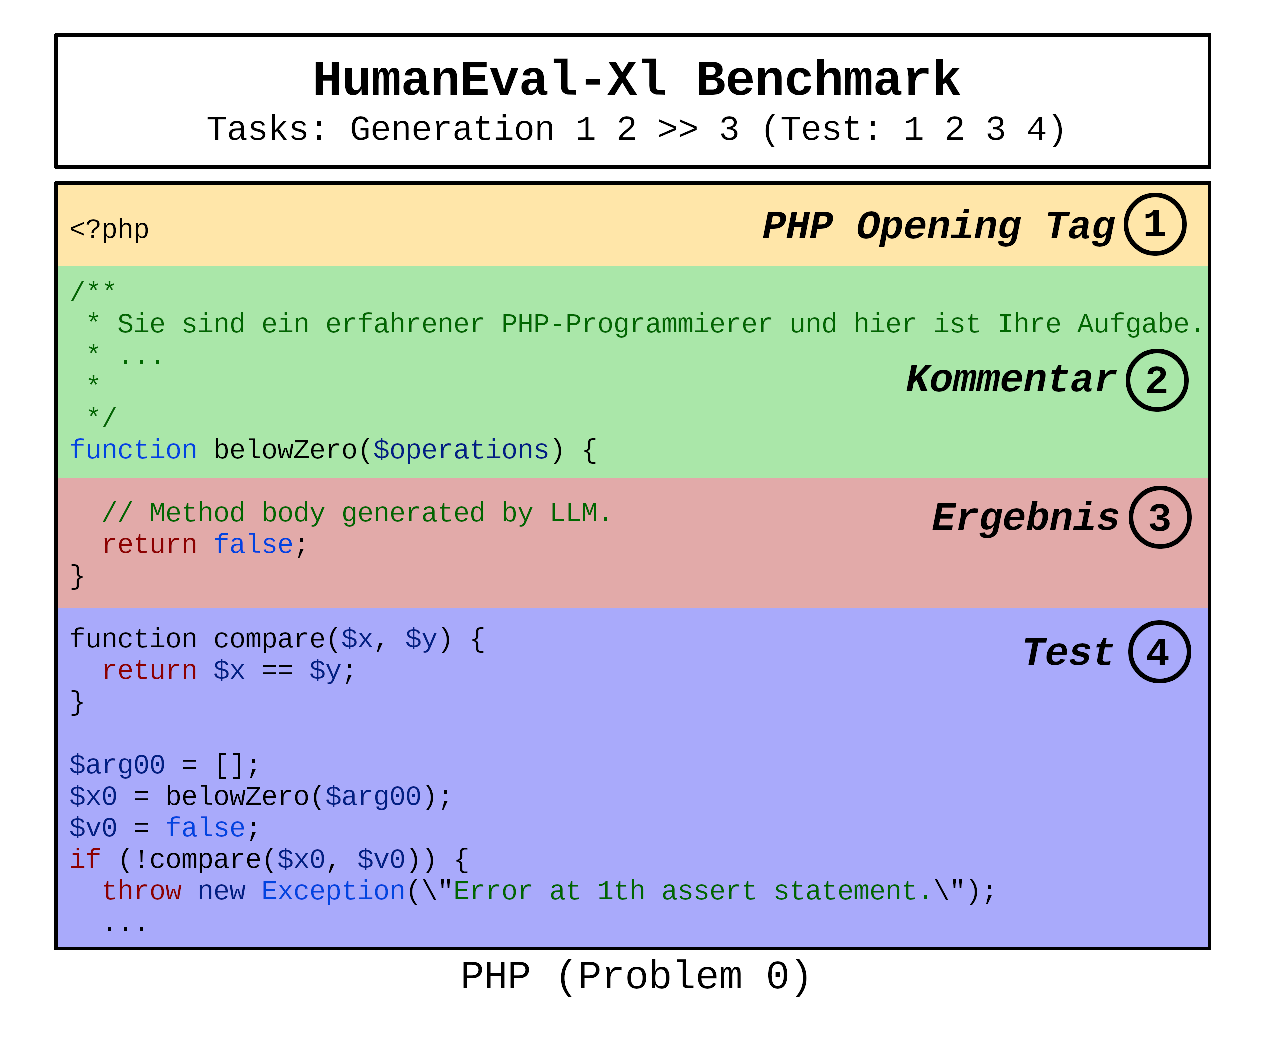
\includegraphics[width=0.6\textwidth]{content/chapter_concept_design/images/code_generation_humaneval_x.eps}
	\centering
	\caption{Aufbau des HumanEval-XL Benchmarks}
	\label{img:code_generation_humaneval}
\end{figure}

Das \textit{PHP Opening Tag}, in der Abbildung \ref{img:code_generation_humaneval} mit \textbf{1} bezeichnet, ist eine optionale Angabe zur Programmiersprache und durch den Benchmark vorgegeben. Während bei den PHP-Proben das Opening Tag \texttt{<?php} lautet, ist beispielsweise bei den JavaScript-Proben kein Opening Tag angegeben. Hier beginnt die Probe direkt mit dem Kommentar. Der in der Abbildung \ref{img:code_generation_humaneval} mit \textbf{2} bezeichnete Kommentar, enthält die eigentliche Aufgabe, die das Modell lösen soll. Auch der Kommentar ist vom Benchmark vorgegeben. Die letzte Zeile enthält den Methodennamen als Codevorgabe, der verwendet werden muss, um nach dem Generieren der Antwort abschließend einen Test durchführen zu können. Die Listings \ref{lst:example_probe_1_of_benchmark} und \ref{lst:example_probe_2_of_benchmark} zeigen Beispiele für die beiden Bereiche aus den ersten zwei Proben des Benchmarks.\vspace{0.2cm}

\begin{lstlisting}[
	language=php,
	label=lst:example_probe_1_of_benchmark,
	caption={PHP Beispiele für die erste Probe}
]
<?php

/**
* Sie sind ein erfahrener PHP-Programmierer und hier ist Ihre Aufgabe.
* Sie erhalten eine Liste von Einzahlungs- und Abhebungsvorgängen auf einem Bankkonto, das mit einem Nullsaldo beginnt. Ihre Aufgabe besteht darin, festzustellen, ob zu irgendeinem Zeitpunkt das Guthaben des Kontos unter Null fällt, und an diesem Punkt sollte die Funktion True zurückgeben. Andernfalls sollte sie False zurückgeben.
* >>> below_zero([1, 2, 3])
* False
* >>> below_zero([1, 2, -4, 5])
* True
*
*/
function belowZero($operations){
\end{lstlisting}


\begin{lstlisting}[
	language=php,
	label=lst:example_probe_2_of_benchmark,
	caption={PHP Beispiele für die zweiten Probe}
]
<?php

/**
* Sie sind ein erfahrener PHP-Programmierer und hier ist Ihre Aufgabe.
* Für eine gegebene Liste von ganzen Zahlen soll ein Tupel zurückgegeben werden, das aus der Summe und dem Produkt aller Zahlen in der Liste besteht.
* Eine leere Summe soll gleich 0 und ein leeres Produkt gleich 1 sein.
* >>> sum_product([])
* (0, 1)
* >>> sum_product([1, 2, 3, 4])
* (10, 24)
*
*/
function sumProduct($numbers){
\end{lstlisting}
	
Diese beiden Teile Opening Tag und Kommentar werden an das Modell als Eingabeaufforderung übergeben und dieses generiert den Code, welches als \textit{Ergebnis} von dem Modell zurückgeliefert wird. Das Modell sollte im Idealfall den vorgegebenen Methodennamen aufgegriffen haben und diesen für die Ausgabe des Ergebnisses verwendet. Somit findet sich der Methodenname auch im Bereich \textbf{3} wieder. Ebenfalls werden oft das Opening Tag und der Kommentar durch das Modell übernommen. In der Abbildung \ref{img:code_generation_humaneval} ist das Ergebnis mit \textbf{3} ausgezeichnet. Der Bereich \textbf{4} bildet den letzten Teil des Benchmarks. Der Test ist ebenfalls vom HumanEval-XL Benchmark vorgegeben. Hier wird ein einfacher Vergleich durchgeführt der bei Abweichung von der Vorgabe eine Exception auslöst. Dazu werden an die vordefinierte Methode Parameter übergeben, aus denen der generierte Code eine Lösung errechnet. Diese wird mit einer, durch den Benchmark vordefinierten Lösung abgeglichen. Das Listing \ref{lst:example_test_1_of_benchmark} zeigt den Aufbau des Tests, am Beispiel der ersten Probe des Benchmarks.\vspace{0.2cm}

\begin{lstlisting}[
	language=php,
	label=lst:example_test_1_of_benchmark,
	caption={PHP Beispiele für den Test der ersten Probe}
]
function compare($x, $y) {
	return $x == $y;
}
$arg00 = [];
$x0 = belowZero($arg00);
$v0 = false;
if (!compare($x0, $v0)) {
	throw new Exception("Error at 1th assert statement.");
}
$arg10 = [1, 2, -3, 1, 2, -3];
$x1 = belowZero($arg10);
$v1 = false;
if (!compare($x1, $v1)) {
	throw new Exception("Error at 2th assert statement.");
}
$arg20 = [1, 2, -4, 5, 6];
$x2 = belowZero($arg20);
$v2 = true;
if (!compare($x2, $v2)) {
	throw new Exception("Error at 3th assert statement.");
}
$arg30 = [1, -1, 2, -2, 5, -5, 4, -4];
$x3 = belowZero($arg30);
$v3 = false;
if (!compare($x3, $v3)) {
	throw new Exception("Error at 4th assert statement.");
}
$arg40 = [1, -1, 2, -2, 5, -5, 4, -5];
$x4 = belowZero($arg40);
$v4 = true;
if (!compare($x4, $v4)) {
	throw new Exception("Error at 5th assert statement.");
}
\end{lstlisting}

\subsection{Durchführung der Evaluierung}
Nach der Generierung des Codes durch das Modell werden die Bereiche \textbf{3} (Ergebnis) und \textbf{4} (Test) für die Evaluierung der Probe verwendet. Hierfür werden die Bereiche zusammengeführt und ergeben einen testbaren ausführbaren Code. Die Ergebnisse werden dokumentiert und dienen für Berechnung der Wahrscheinlichkeit, das ein Modell unter $k$-Proben eine korrekte Antwort liefert.\vspace{0.2cm}

Der Ablauf der Evaluation ist in Abbildung \ref{img:sequence_of_evaluation} dargestellt.\vspace{0.2cm}

\begin{figure}[!ht]
	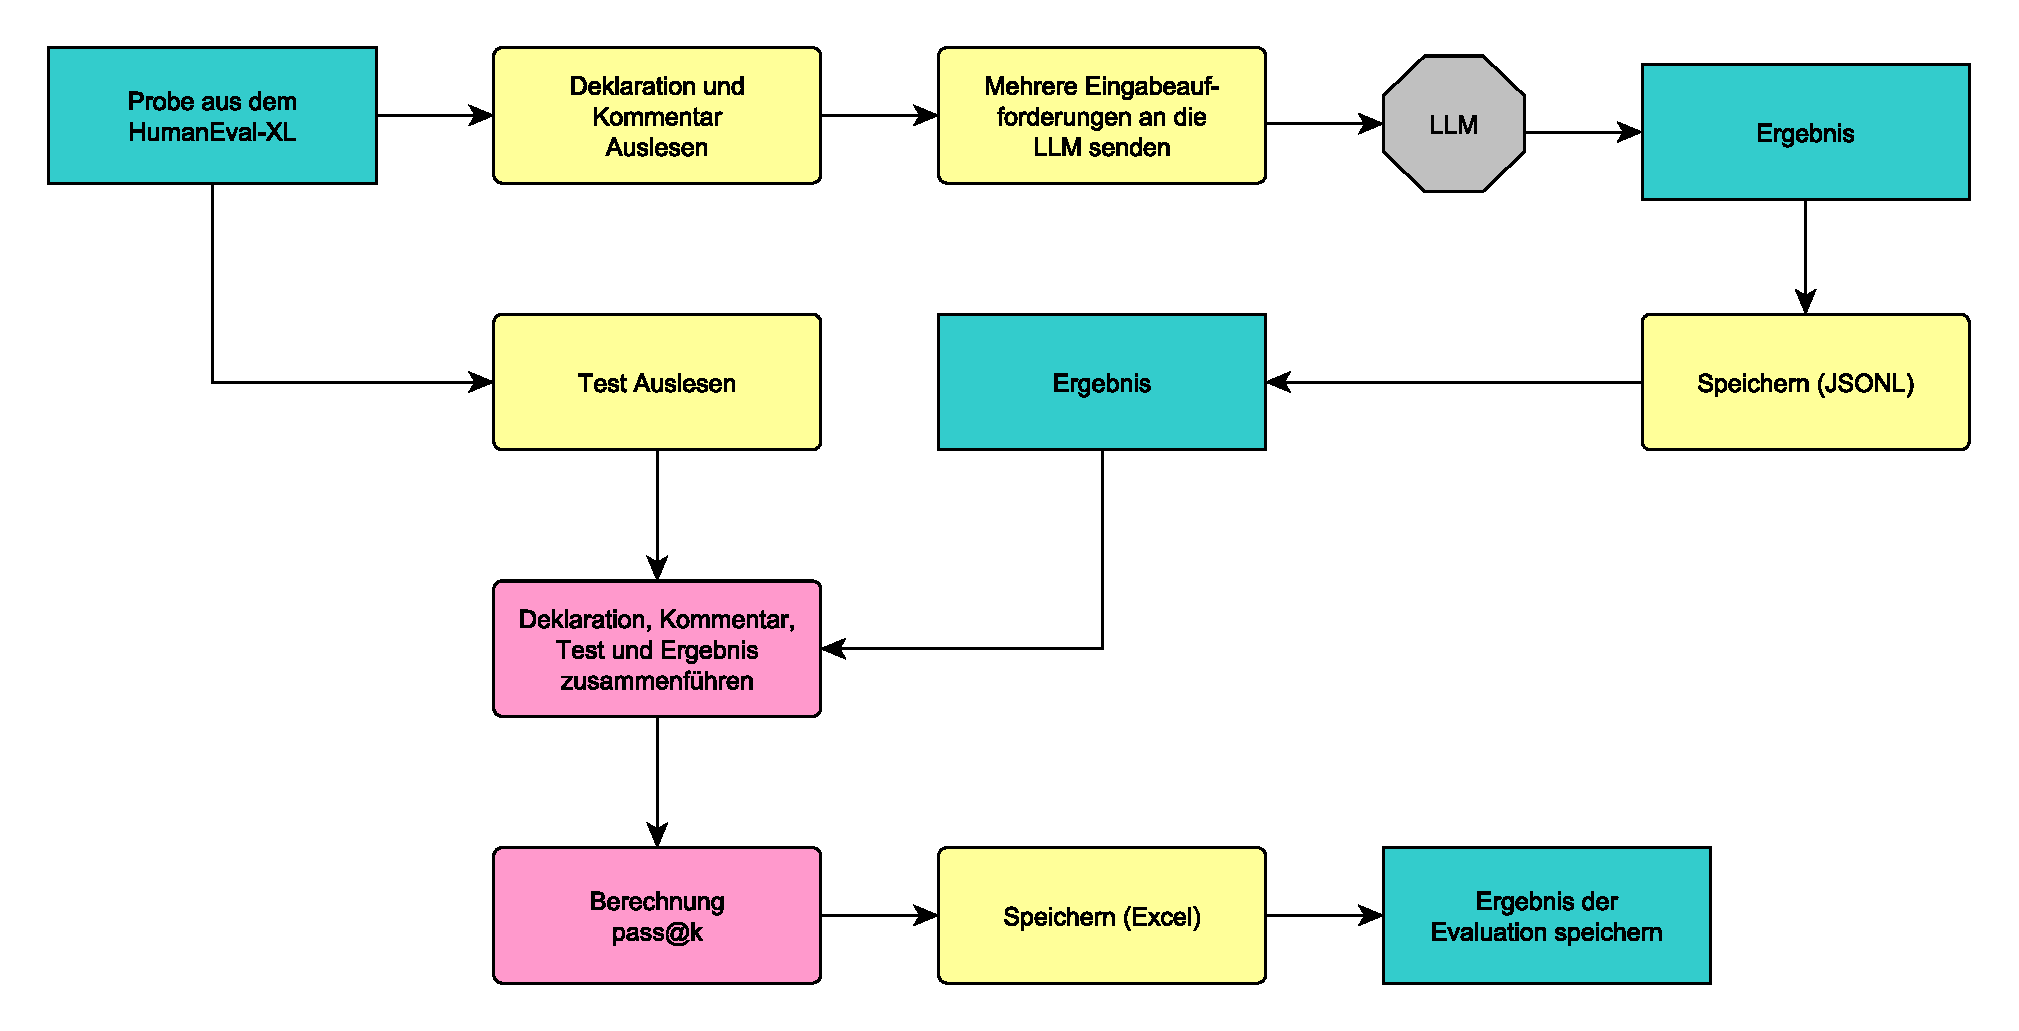
\includegraphics[width=\textwidth]{content/chapter_concept_design/images/ablauf_evaluation.eps}
	\centering
	\caption{Aufbau des HumanEval-XL Benchmarks}
	\label{img:sequence_of_evaluation}
\end{figure}


%*   Welche Arten von Code sollen generiert werden? (z.B. einfache HTML-Formulare, komplexe JavaScript-Funktionen, serverseitiger Code in Python/Node.js, etc.)
Um die Modelle zu evaluieren und ihre Fähigkeiten hinsichtlich der im Web vorherrschenden Programmiersprachen zu untersuchen, werden die Tests in den Programmiersprache PHP und in der deutschen Version vorgenommen. Dafür sollen die Modelle mehrfach einfache Funktionen generieren.\vspace{0.2cm}

%*   Wie werden die Testfälle für die Evaluation generiert? (z.B. manuelle Erstellung, automatische Generierung, Verwendung von bestehenden Code-Snippets, etc.) Wie groß ist der Umfang der Testfälle? (Anzahl der zu generierenden Code-Snippets)
Der Benchmark liefert jeweils einen Test für die Evaluierung mit. Dazu werden bereits in den Prompts die Namen der Methoden und die zu übergebenen Parameter angegeben, welche durch die Modelle zu erstellen sind. Der jeweilige Test verwendet dann diesen Namen und übergibt die geforderten Parameter. Das Listing \ref{lst:example_prompt_test_by_humaneval_benchmark} zeigt ein Beispiel für einen mitgelieferten HumanEval-XL Test.\vspace{0.2cm}

\begin{lstlisting}[language=php,caption={Beispiel für einen Test aus dem HumanEval-XL Benchmark},label=lst:example_prompt_test_by_humaneval_benchmark]
function compare($x, $y) {
	return $x == $y;
}
$arg00 = [3, 1, 2, 4, 5];
$x0 = median($arg00);
$v0 = 3;
if (!compare($x0, $v0)) {
	throw new Exception(\"Error at 1th assert statement.\");
}
\end{lstlisting}


%*   Wie werden die Ergebnisse der LLMs verglichen? (z.B. Vergleich mit Referenzcode, manuelle Überprüfung, automatische Tests, etc.)
Um die Modelle untereinander zu vergleichen, bekommen alle Modelle dieselben Prompts. Von jedem Prompt werden pro Modelle fünf Varianten erstellt. Die Ergebnisse werden in einer Liste chronologisch gespeichert. Mithilfe der pass@k Methode erfolgt die Evaluierung der Ergebnisse und anschließend die Bewertung der Modelle.

\subsection{Dokumentation der Daten}
Die verwendeten Dateien des Benchmarks sind im \textit{JSONL}-Format festgehalten. Ebenso werden die Ergebnisse der LLM Abfragen in diesem Format dokumentiert. Für jede Probe wurde eine separate Datei erstellt, die jeweils fünf Ergebnisse einer LLM enthält. Für den gesamten Benchmark sind pro LLM 80 \textit{JSONL}-Dateien vorhanden.\vspace{0.2cm}

Neben den Rohdaten wurden die Ergebnisse in verschiedenen \textit{Open Document Speadsheet} (ODS) übernommen. Die Dateien lassen sich mit Tabellenkalkulationstool von OpenOffice oder LibreOffice öffnen. Dies dient als Zusammenfassung der Ergebnisse und Zusätzlich wurden hieraus Grafiken generiert, welche auch in diesem Dokument Verwendung finden.\vspace{0.2cm}

Als letztes wurden die programmierten Klassen und Methoden in Python-Dateien (\texttt{*.py}) abgelegt, mit denen die Ergebnisse erstellt und evaluiert wurden. Somit lasen sich alle erhobenen Ergebnisse nachvollziehen.

%---------------------------------------------------------------------------------------------------


\section{Konzeption der Optimierung}
%*   Welche Strategien für das Prompt-Engineering werden untersucht? (z.B. Few-Shot-Prompting, Chain-of-Thought-Prompting, Verwendung von Code-Kommentaren als Prompts, etc.)
%Während die Evaluierung der Modelle ausschließlich mit den Proben des HumanEval-XL erfolgten, wird die Optimierung der Prompts, an zusätzlichen eigenen erstellten Proben erfolgen. Diese sind komplexer als die allgemeinen Proben aus dem HumanEval-XL Benchmark. Hierbei soll untersucht werden, mit welchem Ansätzen Prompts im Bereich der Codegenerierung für die Webprogrammierung erfolgen kann. Es wird neben der Proben auch ein Unittest vorgegeben. Somit kann die Codeüberprüfung der generierten Snippets mit Unittests erfolgen. Der Vorteil von Unittest ist, dass alle Tests durchgeführt werden, auch wenn ein vorheriger Test fehlschlägt. Um diese Tests ausführen zu können, sind PHP Dateien erforderlich. Somit müssen die generierten Codes in Dateien gespeichert und können im Anschluss geprüft werden.\vspace{0.2cm}

%Für die Evaluierung der Ergebnisse der Optimierung wird manuell und automatisiert erfolgen. Durch die automatisierte Evaluierung ist auch hier der Vorteil gegeben das die Ergebnisse der ausgewählten Modelle nach dem gleichen Verfahren beurteilt werden. Wie bei der Evaluierung der Modelle werden die Ergebnisse auch hier festgehalten und dokumentiert.\vspace{0.2cm}

%In der Arbeit werden verschiedene Möglichkeiten der Optimierung untersucht, die in den folgenden Kapiteln vorgestellt und deren Durchführung erläutert werden.


%\subsection{Prompt-Engineerings}
Die Prompts aus dem HunamEval-XL Benchmark sind als \textit{One-Shot-Prompts} oder \textit{Few-Shot-Prompts} verfasst. So sind neben der eigentlichen Aufgabe, noch ein oder mehrere Beispiele für die Eingabeparameter der geforderten Methode und das erwartete Ergebnis angegeben. Das Listing \ref{lst:example_prompt_by_humaneval_benchmark} zeigt ein Beispiel für einen Prompt aus dem HumanEval-XL Benchmark. Im gezeigten Beispiel wird die Aufgabe und zwei Lösungsbeispiele als Prompt an die LLM gesandt. Die Beispiele enthalten die Eingabeparameter und das geforderte Ergebnis der erwarteten Methode.\vspace{0.2cm}

\begin{lstlisting}[language=php,caption={Prompt Beispiel für  eine Aufgabe aus dem HumanEval-XL Benchmark},label=lst:example_prompt_by_humaneval_benchmark]
<?php
/**
 * Sie sind ein erfahrener PHP-Programmierer und hier ist Ihre Aufgabe.
 * Gib den Median der Elemente in der Liste l zurück.
 * >>> median([3, 1, 2, 4, 5])
 * 3
 * >>> median([-10, 4, 6, 1000, 10, 20])
 * 15.0
 */
function median($l){
\end{lstlisting}

Anders als bei \textit{Zero-Shot-Prompts}, können LLMS durch die Angabe von Beispielen die Regeln besser erlernen, Muster und Konzept der Aufgabe besser verstehen und es wird eine Verbesserung des generieren Programmcodes erreicht. Durch das Anwenden der Art von Prompts Design wurden die Eingabeaufforderungen bereits durch die Autoren des HumanEval-XL optimiert.\vspace{0.2cm}

Neben der Optimierung des Prompt Designs wurde weitere Optimierungen in den Eingabeaufforderungen des HumanEval-XL angewandt. So wurde die Eingabeaufforderung bereits als Kommentar der jeweiligen Programmiersprache verfasst. Bei der Probe für die PHP Programmierung wird vor dem Kommentar auf das, für PHP Programme erforderliche . Das definiert einen Kontextparameter und liefert für die LLM einen ersten Anhaltspunkt der zu generierenden Programmiersprache.\vspace{0.2cm}

Eine weitere Optimierung der Eingabeaufforderung ist die letzte Zeile. Hier ist bereits der Name für die erwartete Funktion angegeben. Hier wird die Fähigkeit der Modelle ausgenutzt, Funktionen und Codes zu vervollständigen. Dies ist wichtig, da die Tests im Benchmark auf einen existierenden Funktionsnamen angewiesen sind.\vspace{0.2cm}

Somit lässt sich feststellen, dass die Eingabeaufforderungen weitestgehend optimiert sind. Daher wird auf eine Optimierung der Eingabeaufforderung verzichtet. Es gibt viele Arbeiten, die sich mit genau diesem Problem befassen und es sind durchaus weitere Möglichkeiten vorhanden, die Eingabeaufforderungen zu optimieren.\vspace{0.2cm}

%*   Wie werden die Prompts aufgebaut sein? (z.B. klare Anweisungen, Beispiele, Kontextinformationen, etc.)
%Bei der Optimierung der Eingabeaufforderungen werden die LLMs bei NL2Code Generierung einen objektorientierten Ansatz zu generieren. Diese generierten Klassen lassen sich mit Test-Frameworks wir \textit{phpunit} und \textit{phpmetrics} evaluieren.\vspace{0.2cm}

\subsection{Optimierung durch Frameworkauswahl}
Eine andere Methode zur Optimierung der Eingabeaufforderungen ist die Verwendung verschiedener Frameworks. Hierbei werden die Eingabeaufforderungen auf verschiedenen Arten und Weisen, je nach Framework angepasst und mit zusätzlichen Meta Angaben versehen. Es soll untersucht werden wie sich die Verwendung unterschiedlicher Frameworks auf die Ausgaben der Modelle auswirkt. In der Arbeit werden die Auswirkungen auf die Ergebnisse der Python-Frameworks \textit{langchain} und \textit{DSPy} für verschiedene Modelle verglichen. Für einen automatisierten Test wird hier der HumanEval-XL angewandt.\vspace{0.2cm}

Das Framework \textit{langchain} wurde 2022 vorgestellt und ermöglicht Nutzern die Entwicklung komplexer Anwendungen für LLMs. Jedoch ist Fachwissen im Prompt-Engineering erforderlich, um optimale Eingabeaufforderungen an die Modelle zu stellen. Dieses Fachwissen ist beim \textit{DSPy}-Framework nicht mehr notwendig. Hier übernimmt das Framework die Optimierung der Eingabeaufforderungen für die Modelle und macht somit das manuelle optimieren der Prompts und deren Techniken überflüssig. \textit{DSPy} ist im Oktober von Forschern veröffentlicht worden die Standards für NLP arbeiten.\vspace{0.2cm}


%*   Werden verschiedene Prompt-Varianten für die gleichen Code-Generierungsaufgaben verwendet, um deren Einfluss auf die Ergebnisse zu untersuchen?
\subsection{Evaluierung der Optimierungen}
Wie auch schon bei der Evaluierung der Modelle werden die Ergebnisse festgehalten, um diese nachvollziehen zu können. Die erhobenen Rohdaten werden in Dateien, die im \textit{JSONL}-Format vorliegen gespeichert. Für die Auswertung der Ergebnisse ist auch hier das \textit{Open Document Speadsheet (ODS)} vorgesehen.\vspace{0.2cm}

Die erstellen Programme für die Erstellung der Rohdaten und der Evaluierung, sind als Python-Dateien \texttt{*.py} abgelegt, um die Nachvollziehbarkeit der Ergebnisse zu gewährleisten.
%Für die erweiterte Messung des PHP Codes kommt das Tool \texttt{phpmetrics} zum Einsatz. \texttt{phpmetrics} liefert eine Vielzahl an Metriken,mit der der Code analysiert werden kann. Bei diesem Tool liegt der Fokus auf die Ergebnisse von \texttt{Cyclomatic Complexity}, mit der die Komplexität des Codes gemessen wird. Auf den \texttt{Maintainability Index} zur Auswertung der Wartbarkeit. Diese ermittelt wie aufwändig es zukünftig ist den Code zu erweitern und bewertet die Lesbarkeit. Ein weiterer Parameter welcher hilft die Komplexität zu bewerten, ist der \texttt{Logical Lines of Code} Parameter. Ein weiteres Indiz zur Wartbar- und Lesbarkeit ist der \texttt{Method Length} Parameter. Ein weiterer Parameter zur Bewertung der Lesbarkeit ist der Parameter \texttt{Numbers of Parmeters}. Diese gibt die Anzahl der Parameter welche in die Methode übergeben werden. Eine hohe Anzahl kann ein Indiz dafür sein, das der Code schwerer zu lesen ist. Zur Bewertung der Dokumentation wird der Parameter \texttt{Comment Density} herangezogen.
%Mithilfe eines Python-Skripts wird der generierte Code mit \texttt{phpmetrics} evaluiert.\vspace{0.2cm}

%(SonarQube, wenn die Zeit es noch erlaubt)

%Mit dem SonarQube steht ein Auswertungstool zur Verfügung, welches neben qualitativen Codeanalyse noch eine Sicherheitsanalyse des Codes durchführt und die technischen Schulden ermittelt. Somit ist SonarQube eine Ergänzung zu \texttt{phpmetrics}. SonarQube wird eine lokale VM ausgeführt und mittels Integration werden die generierten Codes an den Server übermittelt.\vspace{0.2cm}

%Beide Verfahren \texttt{phpmetrics} und \texttt{SonarQube} benötigen für die Analyse Dateien. Somit müssen die Ergebnisse erst als Datei gespeichert werden, bevor die Tools mit der Analyse beginnen.


%*   Dieser Abschnitt ist besonders wichtig, da er sich mit der Optimierung der LLMs durch Prompt-Engineering beschäftigt.

%---------------------------------------------------------------------------------------------------


\section{Testumgebung}
%*   Welche Hardware und Software werden für die Experimente verwendet? (z.B. CPU, GPU, Betriebssystem, Programmiersprachen, Bibliotheken, etc.)
Die \textit{Open-Source}-Modelle laufen auf einem Debian 12 System, welches mit 8 Kernen (16 Threads) und 32 GB RAM ausgestattet ist. Um zusätzlichen Speicher zu erhalten, wurde eine 100 GB Swap Partition genutzt. Zur Unterstützung wurde eine RTX 3060 Grafikkarte der Firma Nvidia, 12 GB VRAM verbaut. Für die Bereitstelle ist das freie Framework Ollama zum Einsatz gekommen.\vspace{0.2cm}

Über die Hard- und Softwarekomponenten der kommerziellen \textit{Cloused-Source}-Modelle sind keine Hardwarespezifikationen oder andere tiefer gehende Informationen vorhanden. Da die Performance für die Evaluierung keine entscheidende Rolle spielt, wird nicht weiter und tiefer gehend recherchiert. \vspace{0.2cm}

Alle wichtigen Codes und Codesequenzen, sowie die Ergebnisse sind im Dokument oder im Anhang zu finden. Der gesamte Code und Ergebnisse sind dokumentiert, sodass die Möglichkeit besteht die Evaluierungen nachzuvollziehen. Alle Daten und Dateien werden unter \href{https://github.com/willi-pahl/master-thesis}{https://github.com/willi-pahl/master-thesis} bereitgestellt.\vspace{0.2cm}

%*   Wie wird die Reproduzierbarkeit der Experimente sichergestellt? (z.B. Verwendung von Versionskontrolle, Dokumentation der Umgebung, etc.)



\chapter{Implementierung}\label{chap:implementation}
\begin{tcolorbox}[
	enhanced,
	colback=red!5!white,
	colframe=red!75!black!50,
	title= Mein roter Faden
	]
	Wichtigsten Aspekte und Schritte der Implementierung. Aufbau und Struktur evtl. Programme, wichtige techn. Entscheidungen (Nicht den gesamten Quellcode abbilden, wenn überhaupt dann im Anhang). Einbinden, nur wenn,

	\begin{enumerate}
		\item Nur erklärungsbedürftigen Code ca. 5-20 Zeilen.
		\item Für Nachvollziehbarkeit.
		\item Kommentare für Erklärung.
		\item Keine Standards oder Bibliotheken.
		\item Komplexe Klassen/Strukturen besser beschreiben.
		\item Alternativen:
		\begin{itemize}
			\item Pseudocode.
			\item Diagramme.
			\item Erklären der Logik durch Text.
		\end{itemize}
	\end{enumerate}

	Max. 10-12\% des Kapitels, Rest in Anhang.
\end{tcolorbox}

\section{Lokale Modelle}
Um die Modelle testen zu können ist es erforderlich diese auf geeignete Hardware bereitzustellen. Die zur Verfügung stehende Hardware erlaubt die Bereitstellung von Modellen bis etwa 70b, wobei hier eine Modellquantisierung angewandt werden muss, sodass die Speichergröße etwa eine maximale Größe von 25 bis 30 Gigabyte nicht überschreitet.\vspace{0.2cm}

Ein Tool zur Verwaltung und Ausführung von LLMs ist Ollama. Ollama bieten eine Reihe von Modellen an, die den zur vor genannten Bedingungen entsprechen. Ein weiterer Vorteil für Ollama ist Unterstützung der Programmiersprache Python. Diese wird verwendet, um mit den Modellen zu interagieren und die Ergebnisse zu evaluieren.


\subsection{Bereitstellen er Modelle}
Für das Testen der lokalen Modelle wird das Ollama Framework angewandt. Dies ermöglicht eine Anbindung an einer API, welche sich beispielsweise mittels Python abfragen lässt. Auf dieser Weise lassen sich Modelle von der \href{https://ollama.com/search}{Ollama Modell} Seite testen. Dazu wird Ollama auf dem Server installiert und konfiguriert, siehe Anhang \ref{sec:install_config_ollama_local}. Nach dem Download stehen die Modelle zur Verfügung und mittels der integrierten API können Interaktionen erfolgen. Das Listing \ref{lst:python_connect_ollama} zeigt die erforderlichen und optionalen Parameter für eine einfache Interaktion mit einem Ollamaserver notwendig sind.\vspace{0.2cm}

\begin{lstlisting}[
	language=Python,
	caption={Interaktion in Python mit Ollamaserver},
	label=lst:python_connect_ollama
]
from langchain_ollama.llms import OllamaLLM

model = OllamaLLM(
    base_url="192.168.1.56:11434", # required
    model="deepseek-r1:32b", # required
    temperature=0.2, top_p=0.95, num_predict=2048, # optional
)
\end{lstlisting}

Zusätzlich bietet Ollama die Möglichkeit ein grafisches Tool zum Testen zu installieren. Mit Open WebUI wird ein Browser basierendes Toll eingesetzt, dass auf dem Ollama-Server aufgesetzt wird. Nach der Installation ist das Tool einsatzbereit und im lokalen Netzwerk, unter http://<<server-ip>>:<<webui-port>> erreichbar. Die Installation wird im Anhang \ref{sec:open_webui} beschrieben.


%\subsection{Modellbereitstellung als Datei}
%Eine zweite Methode zur Bereitstellung von Modellen die für diese Arbeit Verwendung findet, ist die direkte Nutzung als lokale Datei. Diese können dann direkt angesprochen werden, in dieser Arbeit wird Python verwendet. Hierbei wurden die Modelle von Hugging Face fokussiert. Diese lassen sich unter anderem mit dem Python Framework \href{https://pypi.org/project/langchain/}{Longchain} orchestrieren.\vspace{0.2cm}

%Nachdem die Modelle von Hugging Face heruntergeladen und lokal abgespeichert wurden, sind diese ohne größeren Aufwand anwendbar. Ein Beispiel für ein mögliches Download-Skript ist in Anhang \ref{sec:hugging_face_models} im Listing \ref{lst:download_hugging_face_model_by_cache} und \ref{lst:download_hugging_face_model} zu sehen. Hierbei ist zu beachten das genügend freier RAM zur Verfügung steht, um die Modelle abzuspeichern.

%-------------------------------------------------------------------------------------------


%\subsection{Orchestrierung von Modellen}
%Die Orchestrierung der Modelle erfolgt mithilfe des Python-Frameworks Longchain. Hierbei werden an die Modelle verschiedene Anforderungen gestellt. Zum einen müssen die Modelle Code generieren, zum anderen ist die Anforderung Text zu erstellen oder zu überarbeiten. Die Abbildung \ref{img:orchestration_llms} zeigt schematisch den Aufbau der orchestrierten Modelle. Der Textfilter sucht in der Ausgabe des ersten Modells den Prompt und eliminiert die Anweisungen und Erklärungen.

%\begin{figure}[!ht]
%	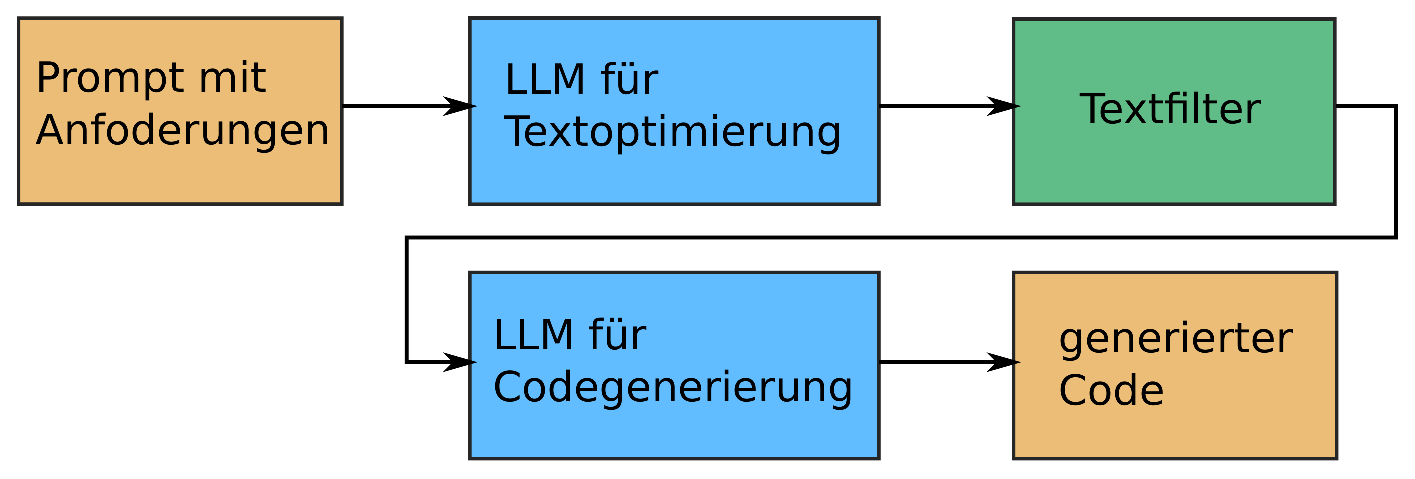
\includegraphics[width=0.8\textwidth]{content/chapter_implementation/images/orchestrierung_llms.eps}
%	\centering
%	\caption{Orchestrierte LLM's für die Codegenerierung}
%	\label{img:orchestration_llms}
%\end{figure}

%\section{Online Modelle}
%Text.

\subsection{Ergebnisse generieren}
Nachdem die Modelle bereitstehen, erfolgt das Generieren der Ergebnisse für jedes einzelne Modell. Mit Prompts, die aus den Proben des HumanEval-XL Benchmark bestehen, werden die Modelle mehrmals hintereinander abgefragt. Die vollständig generierten Antworten der Modelle werden, für eine spätere Auswertung und Nachvollziehbarkeit im \textit{JSONL}-Dateiformat gespeichert. Für jedes Problem erfolgen fünf Abfragen an jedes Modell. Welche Modelle für die Generierung verwendet wurden, ist in Kapitel \ref{subsec:llm_selection} nachzulesen. Alle Modelle wurde von Ollama-Framework bereitgestellt. Das Listing \ref{lst:python_generation_code} zeigt eine einfache Eingabeaufforderung, die an ein Modell gesandt wird.\vspace{0.2cm}

\begin{lstlisting}[
	language=Python,
	caption={Interaktion in Python mit Ollamaserver},
	label=lst:python_generation_code
]
from langchain_ollama.llms import OllamaLLM
from langchain.prompts import PromptTemplate

sample = read_sample_by(task_id=task_id)

model: OllamaLLM
answers: list = []
template = PromptTemplate(
    input_variables=["prompt"],
    template="{prompt}"
)
prompt = template.invoke({"user_prompt": sample.get("prompt")})

for index in range(0, 5):
    answers.append(model.invoke(prompt))

write_result(sample=sample.get("task_id"), answers=answers)
\end{lstlisting}

Nachdem die Proben in Zeile vier vom HumanEval-XL Benchmark eingelesen sind, wird in Zeile sechs bis zwölf das Modell und das Prompttemplate initialisiert. Um die Information \texttt{sample.get("prompt")} aus den Proben zu lesen, wird hier auf den Aufbau der Proben hingewiesen der in Kapitel \ref{subsec:structor_of_humaneval_xl} beschrieben wurde. Anschließend wird das Modell fünfmal abgefragt, hieraus lassen sich später, nach der \texttt{pass@k}-Methode, mit \texttt{k=\{0,...,5\}}, die Modelle evaluieren. Zum Schluss werden die Ergebnisse wie in Zeile siebzehn gezeigt, in JSONL-Dateien abgespeichert.

%---------------------------------------------------------------------------------------------------


\section{Optimierung der Antworten durch Änderung des Frameworks}
Wie das \texttt{langchain} Framework basiert das \texttt{DSPy} ebenfalls auf Python und eignet sich für die Abfrage lokale Ollama Modelle. Somit kann der vorhandene Ollama-Server genutzt werden.
Das Listing \ref{lst:python_generation_code_with_dspy} zeigt die einfache Initialisierung einer Interaktion mit einem lokalen Ollama Models mithilfe der \texttt{DSPy} Bibliothek.\vspace{0.2cm}

\begin{lstlisting}[
	language=Python,
	caption={Interaktion in Python mit Ollamaserver},
	label=lst:python_generation_code_with_dspy
]
import dspy

class BasicProgramming(dspy.Signature):
    question = dspy.InputField(desc="Eine Frage zu PHP Programmierung")
    answer = dspy.OutputField(desc="Generiere Programmcode")

model: dspy.LM = dspy.LM(
    api_base="http://192.168.1.56:11434", # required
    model="ollama_chat/deepseek-r1:32b", # required
    api_key="", # required
    temperature=0.2, # optinal
    cache=False, # optinal
    cache_in_memory=False, # optinal
)

dspy.configure(lm=model)
model(messages=[
    {
        "role": "user",
        "content": "Du bist erfahrener PHP Entwickler",
    }
])

chain = dspy.ChainOfThought(BasicProgramming)
\end{lstlisting}

Der Code zeigt Nach dem Bibliotheksimport wird die Signatur für die Abfrage erstellt. Hier wird die Interaktion mit dem Modell definiert. Es wird die erwartete Eingabe (\texttt{question}) und Ausgabe (\texttt{answer}) festgelegt. Die \texttt{desc}-Parameter im \texttt{InputField} und \texttt{OutputField} dienen lediglich für eine Beschreibung der Felder und haben keinen Einfluss auf den generierten Code.\vspace{0.2cm}

Im Anschluss wird das Lokale Modell mit erforderlichen und optionalen Parametern konfiguriert. Die Parameter \texttt{api\_base}, \texttt{model} und \texttt{api\_key} sind erforderlich. Wobei der Wert für \texttt{key} leer bleibt, solang der Ollama-Server keine Keys für die Anmeldung verwendet. Der Zusatz \texttt{ollama\_chat} veranlasst das Modell-Objekt nach einem Ollama-Server unter der, in \texttt{api\_base} angegebenen IP zu suchen. Mit einer \texttt{temperature}-Angabe von \texttt{0.2} wird das Modell zu einer deterministischen Antwort geleitet. Hier ist eine hohe Kreativität nicht gewünscht. Werden die optionalen Parameter \texttt{cache} und \texttt{cache\_in\_memory} nicht gesetzt, so wird ein Cache eingesetzt, was dazu führt, dass die Abfrage nur einmal in die LLM leitet und die Antwort in einem Cache abgelegt wird. Bei allen weiteren Anfragen würde diese Antwort wiederholt zurückliefert. Das würde bedeuten, das immer nur der $pass@k$ für $k=1$ erstellt werden könnte. Um dies zu verhindern, müssen beide Parameter den Wert \texttt{False} erhalten.\vspace{0.2cm}

Nachdem das Modell konfiguriert ist, wird in Zeile 16 DSPy mit dem Modell \texttt{model} konfiguriert und definiert somit deren Verwendung. Ab der Zeile 17 wird dann die Systemnachricht initialisiert. Diese Systemnachricht wird als erste Nachricht an die LLMs gesendet und legt dadurch den Kontext fest.\vspace{0.2cm}

Die letzte Zeile des Listings \ref{lst:python_generation_code_with_dspy} zeigt die Erstellung einer \texttt{ChainOfThought} Instanz mit der zuvor erstellten Signatur.


\subsection{Ergebnisse generieren}
\begin{tcolorbox}[
	enhanced,
	colback=red!5!white,
	colframe=red!75!black!50,
	title= Mein roter Faden
	]
	Mögliche Optimierungsstrategien
	\begin{itemize}
		\item mit dem Model Programming (DSPY) Ansatz: Python Bibliothek vorhanden \href{https://pypi.org/project/dspy/}{pypi.org | DSPy}.
	\end{itemize}
\end{tcolorbox}

%---------------------------------------------------------------------------------------------------


%\subsection{Auswertung der Modellantworten}
\section{Benchmark Codeevaluation}\label{sec:benchmark_evaluation}
Die Analyse der generierten Antworten muss für jedes Modell individuell angepasst werden, da die erzeugten Codefragmente zwischen den Modellen variieren. Insbesondere unterscheiden sich die Formate, in denen die Codesnippets generiert werden, beispielsweise durch \texttt{```php} oder \texttt{```php \textbackslash n <?php}. Dementsprechend erfordert die Extraktion des relevanten Codes aus den Modellantworten eine flexible Methode, die an das jeweilige Ausgabeformat der Modelle angepasst wird. Ein exemplarischer Lösungsansatz zur Extraktion des generierten Codes ist in Listing \ref{lst:code_extraction} dargestellt.\vspace{0.2cm}

\begin{lstlisting}[
	language=Python,
	caption={Codesnippet zur Extrahierung des Codes aus der LLM Antwort},
	label=lst:code_extraction
]
def get_generatet_code(code=code):
    if len(code.split("```php")) > 1: # find start
        code = code.split("```php")[1]
        code = code.split("```")[0]

    if code.startswith("<?php"): # find start
        code = code.split("<?php")[1]
        code = code.split("?>")[0]

    if len(code.split(r"\n}\n")) > 0: # find end
        code = code.split(r"\n}\n")[0] + "\n}\n"

    return code
\end{lstlisting}

Um den generierten Code zu evaluieren, wird dieser zusammen mit dem Test, der jeweiligen Probe aus dem Benchmark zusammengeführt. Das Ergebnis ist ein ausführbarer Code, der die geforderte Methode enthält. Mittels Python wird der Code getestet, ob der dieser ausführbar ist. Entsteht bei der Ausführung ein Laufzeitfehler erfolgt der Abbruch des Tests. Dieser kann ausgelöst werden durch eine nicht korrekte Syntax, einer Endlosschleife oder wenn die geforderte Methode nicht generiert wurde. All diese Ereignisse führen dazu, das die Probe als nicht bestanden gilt. Das Listing \ref{lst:php_interpreter_in_python} zeigt den Ausschnitt im Code zur Ausführung des PHP Interpreters in Python.\vspace{0.2cm}

\begin{lstlisting}[
language=Python,
caption={Codesnippet zur Ausführung des PHP Interpreters},
label=lst:php_interpreter_in_python
]
import subprocess

def test_answer(task_id, repetition):
    # read generated code
    answer = read_answer(task_id=task_id, repetition=repetition)
    answer = get_generatet_code(code=answer)

    # read test in HumanEval-XL
    test = read_sample(task_id=task_id).get("test")

    try:
        result = subprocess.run(
            ["php", "-r", f"{test}{answer}"],
            capture_output=True,
            text=True,
            check=False,
            timeout=5,
        )
    except subprocess.TimeoutExpired:
        return False

    if result.stderr.strip() == "":
        return True

    return False
\end{lstlisting}

Nachdem eine von fünf Antworten des Modells und der Test aus dem Benchmark vorliegen, erfolgt die Prüfung des generierten Codes. Diese wird im Listing \ref{lst:php_interpreter_in_python} ab Zeile zwölf gezeigt. Die Funktion liefert \texttt{True} zurück, wenn es keine Fehler im Test gab, sonst immer \texttt{False}. Das Exception-Handling ab Zeile 19 wird aufgerufen, wenn die PHP Ausführung in einer Schleife hängt. Hier wird ein \texttt{Timeout} abgefangen und somit gibt der Test als nicht bestanden. Aus den erhaltenen Ergebnissen, der Proben eines Tasks, berechnet die \texttt{pass@k} Methode, die \glqq Wahrscheinlichkeit das in \texttt{k}-Proben, eine korrekte Probe ist\grqq \, hinsichtlich Codegenerierung. Anschließend wird der Durchschnitt für die Zuverlässigkeit des Modells errechnet.\vspace{0.2cm}

\textbf{Umsetzung der pass@k Metric}\vspace{0.2cm}

Nach Abschluss der Tests werden die Ergebnisse mithilfe der \textit{pass@k}-Methode analysiert. In Python steht hierfür, die Bibliothek \textit{pass\_at\_k} zur Verfügung. Das Listing \ref{lst:custom_pass_at_k} zeigt die Implementierung der Methode gemäß Gleichung \ref{equ:pass_qt_k_complex} in Kapitel \ref{subsec:pass_at_k}, wie sie auch in der Python-Bibliothek verwendet wird.  


\begin{lstlisting}[
	language=Python,
	label=lst:custom_pass_at_k,
	caption={Berechnung der pass@k Metrik in Python}
]
def custom_pass_at_k(n: int, c: int, k: int) -> float:
    """
    :param n (int): numbers of total samples.
    :param c (int): number of currect samples.
    :param k (int): number of consider samples.
    """
    if n - c < k:
        return 1.0
    return 1.0 - np.prod(1.0 - k / np.arange(n - c + 1, n + 1))
\end{lstlisting}

%Die \textit{pass@k}-Methode dient zur Berechnung der Wahrscheinlichkeit, dass in $k$ Abfragen mindestens eine korrekte Lösung enthalten ist. Dazu
Die Methode erwartet drei Parameter. Der Parameter $n$ bezeichnet die Gesamtanzahl der Abfragen pro Probe. Der Parameter $c$ gibt die Anzahl der korrekten Abfragen innerhalb einer Probe an. Schließlich legt der Parameter $k$ fest, wie viele der besten Abfragen für die Bewertung berücksichtigt werden. Alle drei Parameter sind ganzzahlig (\texttt{Integer}), während das Ergebnis als Gleitkommazahl (\texttt{Float}) zurückgegeben wird.  

In dieser Arbeit werden die Werte $k=1$ und $k=5$ für die Evaluierung herangezogen. Nachdem jede Probe des HumanEval-XL-Benchmarks einzeln bewertet wurde, wird eine aggregierte Bewertung für das gesamte Modell ermittelt. Diese Berechnung erfolgt gemäß Gleichung \ref{equ:probability_of_success_per_model} in Kapitel \ref{subsec:pass_at_k}.  

% --- More Tests -----------------------------------------------------------------------------------


%\section{Codeevaluation mit Frameworks}
%Neben der bekannten Evaluationsmethode mit dem HumanEval Benchmark, wird hier eine weitere Testmethodik überprüft, die mit verschiedenen Validierungstools der jeweiligen Programmiersprache ausgeführt wird. Für die Erstellung der Abfragen wird das Python-Skript verwendet, was schon im Kapitel \ref{sec:benchmark_evaluation} vorgestellt wurde.

%\subsection{PHP Codeevaluation}
%Der Test wird bei den erweiterten Problemen durchgeführt und beginnt mit den Unit-Tests die mit \textit{PHPUnit} durchgeführt werden. Im Anschluss wird \textit{PHPMetrics} ausgeführt. Hierbei wird geprüft, ob die Codekomplexität und Wartbarkeit überprüft. Die Ausführung der Tests wird mithilfe eines Python-Skripts durchgeführt. Es wird eine PHP Datei erstellt, die mit den Frameworks geprüft wird.

%\subsection{JavaScript Codeevaluation}
%Text.

%\section{Online Modelle}
% Eigenen KI Server \href{https://www.computerweekly.com/de/ratgeber/Einen-KI-Server-mit-Ollama-und-Open-WebUI-einrichte}{Computer Weekly}
% Orchestrierung mit Python \href{https://pypi.org/project/multillm/}{multillm-Projekt}
% LangChain Library \href{https://python.langchain.com/api_reference/ollama/chat_models/langchain_ollama.chat_models.ChatOllama.html}{Example}
% \href{https://pypi.org/project/langchain-ollama/}{Python lib langchain-ollama}
% YouTube \href{https://www.youtube.com/@AICodeKing}{AICodeKing}

\chapter{Evaluation}\label{chap:evaluation}
Die Evaluation der Ergebnisse erfolgt im ersten Schritt anhand des HumanEval-XL Benchmarks. Dieser Benchmark wird in \cite{peng-2024} vorgestellt und erweitert den HumanEval \cite{chen-2021}. Der HumanEval-Benchmark evaluiert nur Python während der HumanEval-XL weitere Programmiersprachen und in verschiedenen Landessprachen unterstützt, darunter auch die deutsche Sprache. Neben Python sind auch Prompts für PHP und JavaScript enthalten, welche für die Webentwicklung wichtig sind. Die Datensätze des HumanEval-XL sind unter \href{https://github.com/FloatAI/humaneval-xl}{https://github.com/FloatAI/humaneval-xl} einsehbar und bestehen jeweils aus 80 Tests. Für jedes Problem werden zehn Lösungsvorschläge generiert, die im Anschluss auf die Aspekte der Syntaktik und Semantik evaluiert werden.\vspace{0.2cm}

Diese Tests fordern LLM's auf kleine Problem zu lösen. Aus diesem Grund werden weitere Tests erstellt mit umfangreicheren Anforderungen aus dem Bereich der Webentwicklung. Zu jedem Problem wird eine Musterlösung und ein Unittest erstellt. Der Aufbau für diese Bereitstellung orientiert sich an dem Format aus dem HunamEval-Benchmark.\vspace{0.2cm}

\begin{tcolorbox}[
	enhanced,
	colback=red!5!white,
	colframe=red!75!black!50,
	title= Mein roter Faden
	]
	Der nachfolgende Absatz wird sich noch mal ändern.  Je nachdem wie Aufwendig eine automatisierte Prüfung umsetzbar ist bzw. sich überhaupt automatisieren lässt.\vspace{0.2cm}
	
	Evtl. manuelle Auswertung von Stichproben.
\end{tcolorbox}

Des Weiteren ist die Bewertung der Coding-Standards der jeweiligen Programmiersprache vorgesehen. Für die Prüfung der Standards wird ein SonarQube-Server verwendet, der sowohl PHP als JavaScript unterstützt. Ebenfalls wird die Qualität des Codes evaluiert. Das Augenmerk liegt auf die Lesbarkeit, Effizienz und Wartbarkeit des generierten Codes.\vspace{0.2cm}

%Optional werden einige Tests von zusätzlichen Tools validiert, beispielsweise bei der Validierung von PHP Files sind es Tools wie phpunit\footnote{phpunit steht unter \href{https://github.com/sebastianbergmann/phpunit}{https://github.com/sebastianbergmann/phpunit} zum Download bereit.} und Code\_Sniffer\footnote{Code\_Sniffer steht unter \href{https://github.com/squizlabs/PHP_CodeSniffer}{https://github.com/squizlabs/PHP\_CodeSniffer} zum Download zur Verfügung.} für die Validierung von JavaScript findet das Framework Jasmin\footnote{\href{https://jasmine.github.io/}{https://jasmine.github.io}.} Anwendung.\vspace{0.2cm}


\section{Bewertung der Modelle}
Für die Bewertung wird das Vorgehen gewählt, welches in \cite{chen-2021} und \cite{peng-2024} beschrieben ist. Die Tests werden exemplarisch, mit den für die Webentwicklung relevanten Sprachen PHP und JavaScript durchgeführt. Die Evaluierung der Modelle wird auf den Ebenen \glqq einfache Fragen\grqq \ und \glqq komplexe Aufgaben\grqq \ erfolgen. Die \glqq einfachen Fragen\grqq \ werden bereits durch den zuvor genannten Benchmarks abgedeckt, sodass der entwickelte Fragenkatalog sich auf die Ebenen mit den \glqq komplexen Aufgaben\grqq \ konzentriert.\vspace{0.2cm}

Aus Ergebnisse der Tests, wird mithilfe der $pass@k$-Metrik, die Zuverlässigkeit der jeweiligen Modelle berechnet. Dieser Wert gibt an, mit welcher Wahrscheinlichkeit mindestens eine richtige Lösung unter $k$ ausgewählten Vorschlägen vorhanden ist. Die Formel \ref{equ:pass_qt_k} zeigt die Berechnung der $pass@k$-Metrik.

\begin{equation}\label{equ:pass_qt_k}
	\text{pass@k} = 1 - \frac{\prod_{i=0}^{n-k} (n - i - c)}{\prod_{i=0}^{n-k} (n - i)}
\end{equation}

Dabei ist $n$ die Gesamtanzahl der Versuche, $c$ die Anzahl der korrekten Lösungen unter den $n$ Versuchen und $k$ gibt die Anzahl der Lösungen an die betrachtet wurden.

%--- Optimierung --------------------------------------------------------------------------------


\section{Optimierung der Ergebnisse}
Ein Ansatz zur Optimierung der Ergebnisse ist, ...

% https://ki-techlab.de/ki-news/evaluierung-grosser-sprachmodelle-ein-technischer-leitfaden/

%\begin{tcolorbox}[
%	enhanced,
%	colback=BhtColorYellow!5!white,
%	colframe=BhtColorYellow!75!black,
%	title= HTML Startseite
%	]
%	Text in der Box
%\end{tcolorbox}

%\begin{tcolorbox}[
%	enhanced,
%	colback=BhtGrey!5!white,
%	colframe=BhtGrey!75!black!50,
%	title= ChatGPT 3.5
%	]
% Text in der Box
%\end{tcolorbox}


\chapter{Lessons Learned}\label{chap:lessons_learned}
\begin{tcolorbox}[
	enhanced,
	colback=red!5!white,
	colframe=red!75!black!50,
	title= Mein roter Faden
	]
Dieses Kapitel wird die positiven und negativen Erfahrungen der Kapitel Implementierung und Evaluation auffassen. Die weiteren Kapitel bauen auf die hier gewonnenen Erkenntnisse auf.
\end{tcolorbox}


\section{Erweiterte Codeevaluation}
Bei den vordefinierten Prüfungen der HumanEval Benchmarks, wird geprüft, ob der Code lauffähig ist, nicht aber die Codestruktur oder Kommentare. Ein Problem bei der Nutzung des von der LLM generiertem Code ist, dass Entwickler diesen einfach kopieren und in ihre Programme implementieren. Es wird also nur die Funktionalität des Codes geprüft, nicht aber Strukturen und Kommentare um die Lesbarkeit und Verständlichkeit zu erhöhen. Dieses Vorgehen mag zu schnellen Erfolgen in der Programmentwicklung führen, wird aber beim Refactoring oder Fehlersuche erhebliche Defizite mit sich bringen.\vspace{0.2cm}

Aus diesem Grund sollte der erstellte Code nicht nur auf die Funktionalität geprüft werden. Dafür sollten weitere Test-Frameworks der jeweiligen Programmiersprache zur Anwendung kommen. Es gibt mehrere Frameworks zur Prüfung der Codequalität unter PHP. Zwei bekannte Frameworks die auch in dieser Arbeit Anwendung finden, sind die Frameworks \texttt{phpunit} und \texttt{phpmetrics}. Mit ihnen wird der, durch die LLMs generierten Codes geprüft.\vspace{0.2cm}

Um PHPUnit und PHPMetrics für die Evaluierung zu verwenden, müssen weitere Angaben und Einträge im Benchmark erfolgen. So muss ein PHP-Unittest enthalten sein, dieser kann den einfachen benutzerdefinierten Test ersetzen. Des Weiteren sind die Kriterien für die Metrik Messung, für jeden Test erforderlich. Die Kriterien können wie in Listing \ref{lst:phpmetric_criteria_example} dargestellt, aussehen.

\begin{lstlisting}[language=python,caption={Beispiel für Bewertungskriterien},label=lst:phpmetric_criteria_example]
	criteria = {
		"Lines of code": lambda x: int(x) > 12,
		"Logical lines of code by method": lambda x: float(x) > 7,
		"Lack of cohesion of methods": lambda x: float(x) > 3,
		"Average Cyclomatic complexity by class": lambda x: float(x) > 10,
		"Average Weighted method count by class": lambda x: float(x) > 20,
		"Average bugs by class": lambda x: float(x) > 0.1,
		"Critical": lambda x: int(x) > 0,
		"Error": lambda x: int(x) > 0,
		"Warning": lambda x: int(x) > 0,
		"Information": lambda x: int(x) > 0,
	}
\end{lstlisting}

Mit den erweiterten Tests werden die Benchmarks, um die folgenden Punkte erweitert.

\begin{myitemize}
	\item \textbf{unittest}: Unittests für die geforderte Funktion, unterschied zu den einfachen Tests
	\item \textbf{metrics}: Kriterien für den Metriktest
\end{myitemize}

\subsection{PHPUnit}
Eines der bekanntesten spezielles Framework für Unit-Tests in PHP, was als Industriestandard gilt. Mit diesem Framework können neben der Prüfung auf funktionsfähigen Code auch Randfälle betrachtet und Fehlerbehandlungen im Code getestet werden. Als Grundlage für die Auswahl des Tools wird auf Studie \cite{mohamad-2016} verwiesen.

\subsection{PHPMetrics}
Ein PHP Framework für die Codeanalyse, welches detaillierte Berichte über die Codequalität, Komplexität des Codes und über dessen Wartbarkeit erzeugt. PHPMetrics wird in verschiedenen Arbeiten eingesetzt, um die Codequalität zu ermitteln. So auch in \cite{anggrain-2016}, bei der verschiedene Open Source LMS verglichen werden.

\subsection{SonarQube}
Als letztes Tool soll SonarQube zur statischen Codeanalyse und Codeprüfung zum Einsatz kommen. Es werden verschiedene Programmiersprachen unterstützt, darunter auch PHP und JavaScript. In der Arbeit \cite{da-silva-simoes-2024} wird die Prüfung der Codequalität mit SonarQube, ChatGPT3.5 und ChatGPT4 vergleichen. Als Schlussfolgerung aus dem Ergebnis dieser Arbeit, wird auch hier die Codeanalyse durch eine LLM nicht erfolgen, sondern ebenfalls durch SonarQube.

%\subsection{ESLint}
%JavaScript Tool zur Syntaxfehler-Erkennung, Stil- und Codequalitätsprüfung. Mit diesem Tool kann reines JavaScript als auch Node.js überprüfen. https://arxiv.org/html/2402.14261v1


\chapter{Diskussion und Ausblick}\label{chap:discussion}
\begin{tcolorbox}[
	enhanced,
	colback=red!5!white,
	colframe=red!75!black!50,
	title= Mein roter Faden
	]
	Struktur des Kapitels
	
	\begin{enumerate}
		\item \textbf{Einleitung}: Eine kurze Einführung in die Diskussion und den Ausblick.
		\item \textbf{Zusammenfassung der Ergebnisse}: Eine kurze Übersicht über die wichtigsten Ergebnisse und in Relation mit den Forschungsfragen stellen.
		\item \textbf{Diskussion der Ergebnisse}: Eine Analyse und Interpretation der Ergebnisse. Vergleich mit Stand der Forschung und früherer Arbeiten.
		\item \textbf{Grenzen und Einschränkungen}: Eine Diskussion der Limitationen der Studie. Z.B. begrenzte Datenbasis, Grenzen der eingesetzter Tools und Technik.
		\item \textbf{Impulse für zukünftige Forschung}: Vorschläge für weitere Studien. Verbesserungsmöglichkeiten der Methoden usw. und Zukunft des Forschungsfeldes und evtl. Trends.
		\item \textbf{Praktische Anwendung}: Eine Diskussion der möglichen Anwendungen der Ergebnisse. In welchen Unternehmen und welche realen Anwendungen können die Ergebnisse eingesetzt werden.
	\end{enumerate}
\end{tcolorbox}

Wie in \cite{hartenstein_2024} beschrieben,
\section{Thesen}
% 3. These: Optimierung ohne Modellanpassung, nur Prompt Engineering
Die Erkenntnisse aus den Experimenten dieser Arbeit bestätigen die aufgestellte dritte These (T3) aus Kapitel \ref{sec:goals_of_the_work}. Eine Optimierung der Eingabeaufforderungen für die Webanwendungsentwicklung lässt sich ohne Änderung der Modellparameter erreichen und bewirken eine signifikante Verbesserung der Ergebnisse. Die Modelle wurden bereits mit Programmiersprachen, die für Webanwendungsentwicklung essenziell sind, wie beispielsweise PHP, trainiert und diese Daten, in Form von Programmcode sind in den Modellen abrufbar. Entscheidend hierbei ist die Art und Weise wie die Gestaltung der Eingabeaufforderungen umgesetzt wird. Diese Optimierung erfolgt durch das \texttt{DSPy} Framework für die meisten Modelle automatisch.\vspace{0.2cm}

Dennoch hat das \texttt{DSPy} Framework, auf einige Modelle eine negative Auswirkung. Der generierte Code schnitt in der Evaluation mit den HumanEval-XL Proben schlechter ab. Das legt die Annahme nahe das  

Aus diesem Grund sollte in diesen Fällen weitere Frameworks, wie beispielsweise \textit{AdalFlow} oder \textit{LamaIndex} für die Optimierung in Betracht gezogen werden.\vspace{0.2cm}

% 2. These: Benckmarks sind ungeeignet
Diese Erkenntnis lassen den Schluss zu, dass die zweite These (T2) aus Kapitel \ref{sec:goals_of_the_work} bewiesen wurde. Ein einzelner Benchmark hat nicht ausreichend Aussagekraft, um eine LLMs hinreichend zu bewerten. Diese Benchmark eignen sich dafür einen ersten Eindruck von den Modellen zu erhalten. Wie auch in \cite{zhang-2024} wird die Auffassung vertreten, dass diese Probe grundlegende Codeproblematiken testen, die nicht mit den realen Bedingungen übereinstimmen. In dem Onlineartikel \cite{albrecht-2023} heißt es \glqq \textit{...liefert Code, der zwar nicht immer direkt nutzbar ist, nach einer Überarbeitung aber schon recht überzeugend läuft.}\grqq \ was darauf hindeutet, dass Programmierer andere Anforderungen an LLMs stellen, die zurzeit mit Benchmarks nicht abgedeckt werden können.\vspace{0.2cm}

% 1. These: LLMs effizientere Webanwendungsentwicklung. Wichtig ist die Evaluierung
In den letzten Jahren hat generative KI auch die Arbeit der Entwickler stark beeinflusst. So ist in \cite{focus-online-2025} die Rede von einem Programmierer, der seine Aufgabe ab brach, \glqq \textit{weil er keinen Zugang zu seinem virtuellen Assistenten hatte. ''Ich kann einfach nicht mehr ohne die Hilfe der KI programmieren''}\grqq \ so der Entwickler. So werden KI Anwendungen bei Entwicklern immer beliebter und das gilt auch für den Bereich der Webanwendungsentwicklung. Dabei verwenden viele Entwickler KI Modellen von US Amerikanischen Unternehmen wie Athropic, Google oder OpenAI

\section{Impulse für zukünftige Forschungen}
Ein interessantes Feld für die Forschung ist die Nutzung generativer KI und welche Auswirkungen dies auf das menschliche Denken und Handeln hat. In der Studie \cite{chiriatti-2024} wird von einem System 0 gesprochen, welches neben den bekannten 
\begin{enumerate}
	\item System 1: schnelles,intuitives und automatisches Denken
	\item System 2: langsameres, analytisches und reflektierteres Denken
\end{enumerate}

eingeführt wird. Hierbei handelt es sich um ein Denken, welches die KI für den Menschen übernimmt. Entscheidungen und Daten werden durch die KI übernommen. Ein externes System, ähnlich wie eine USB-Festplatte eines PCs.\vspace{0.2cm}

Inwieweit können auch \textit{Small Language Models} für Programmieraufgaben eingesetzt werden. Könnte der enorme Energiebedarf und Ressourcen der LLMs durch SLMs ersetzt werden? Siehe 
\href{https://medium.com/@nageshmashette32/small-language-models-slms-305597c9edf2}{Small Language Models (SLMs)} oder \href{https://medium.com/version-1/small-but-powerful-a-deep-dive-into-small-language-models-slms-b793bdb002f2}{Small but Powerful: A Deep Dive into Small Language Models (SLMs)}. Eine weitere Forschung kann die Evaluation sein, ob Finetuned SLMs, wie Phi-2, Google Gemini Nano oder Metas Llama-2-13b bessere Ergebnisse liefern, als die LLMs.\vspace{0.2cm}

Ein weiteres Feld kann sich mit der Einführung einer KI in Firmen befassen und Fragen wie,

\begin{itemize}
	\item Wie können Entwickler bestmöglich vorbereitet werden, um die Einführung von KI reibungslos zu ermöglichen?
	\item Wie kann Datensicherheit und Datenqualität sichergestellt werden?
	\item Evaluierung von Kosten/Nutzen für die Einführung von KI in Softwareunternehmen.
\end{itemize}

evaluieren.


%\begin{tcolorbox}[
%	enhanced,
%	breakable,
%	colback=red!5!white,
%	colframe=red!75!black!50,
%	title= Mein roter Faden: noch was zum Testen
%	]
%	Ein Tool zur Orchestrierung von Multi-Agenten-Systemen \href{https://community.openai.com/t/introducing-swarm-js-node-js-implementation-of-openai-swarm/977510}{OpenAI Swarm}, gefunden auf \href{https://karrierewelt.golem.de/blogs/karriere-ratgeber/bot-belegschaft-mit-entlastungspotenzial-ki-agenten-fur-den-arbeitsalltag-in-der-testphase-1}{Golem | Karrierrewelt}.
%\end{tcolorbox}

\section{Praktische Anwendung}
Blaupause für Prompting \href{https://piamedia.com/wp-content/uploads/2024/09/PIAM_Whitepaper_LLM-Halluzinationen_DE.pdf}{Das Geheimnis hinter LLM-Halluzinationen} [S. 16 ff.] noch testen und evaluieren.

\href{https://arxiv.org/html/2501.16998v1}{Große Sprachmodelle zur Codegenerierung: Die Perspektive der Praktiker}

\subsection{Anwendung für Entwickler}
Zur Optimierung des generierten Codes kann auch die freie Wahl der Softwarekomponenten durch die LLMs betragen. Wie in \cite{chen-2021} beschrieben können Nutzer, anstatt in Suchmaschinen beispielsweise die Vorteilen und Nachteile von \texttt{PyTorch} und \texttt{Tensorflow} zu vergleichen, kann das die LLM übernehmen und als Prompt wird nur \texttt{\# import machine learning package} angegeben.\vspace{0.2cm}

Wie in [Quelle ist weg] beschrieben nimmt das Lesen von Programm zehn mal mehr Zeit in Anspruch, als Code zu schreiben. Diese Arbeit kann ebenfalls durch eine LLM übernommen werden.

\chapter{Fazit}\label{chap:conclusion}
\begin{tcolorbox}[
	enhanced,
	colback=red!5!white,
	colframe=red!75!black!50,
	title= Mein roter Faden
	]
	Struktur des Kapitels
	
	\begin{enumerate}
		\item \textbf{Zusammenfassung}: kurze Wiederholung der Zielsetzung d. Arbeit, Überblick der wichtigsten Ergebnisse aus Eval. und Optimierung, Fragestellung beantwortet?
		\item \textbf{Reflexion}: Stärken und Schwachen d. Arbeit, Diskussion über mögliche  Fehlerquellen, Einschätzung Optimierungsansätze oder Benchmarks
	\end{enumerate}
\end{tcolorbox}

\begin{tcolorbox}[
	enhanced,
	colback=red!5!white,
	colframe=red!75!black!50,
	title= Mein roter Faden
	]
	Unterschied Diskussion/Ausblick und Fazit\vspace{0.2cm}
	
	\begin{tabular}{|l|l|l|}
		\hline
		\textbf{Aspekt} & \textbf{Diskussion und Ausblick} & \textbf{Fazit} \\
		\hline
		\textbf{Funktion} & Kritische Analyse und & Zusammenfassung und \\
		& Zukunftsperspektive & Abschluss \\
		\hline
		\textbf{Zeitperspektive} & Zukunftsorientiert & Rückblickend \\
		\hline
		\textbf{Detaillierungsgrad} & Detailreichere Auseinandersetzung & Knapp und prägnant \\
		&  mit Ergebnissen & \\
		\hline
	\end{tabular}\vspace{0.2cm}
	
	Während \glqq Diskussion und Ausblick\grqq \ die Ergebnisse kritisch reflektiert und auf zukünftige Entwicklungen verweist, fasst das \glqq Fazit\grqq \ die Arbeit kompakt zusammen und beantwortet die Forschungsfrage. Beide Kapitel sind komplementär, aber klar voneinander zu unterscheiden.
\end{tcolorbox}

Es gibt Modelle welche besonders für die Webanwendungsentwicklung sehr gute Ergebnisse, auch ohne Optimierung liefern. Dennoch sollte eine Optimierung der Eingabeaufforderungen in Betracht gezogen werden, da diese mit relativ wenig Aufwand umsetzbar ist. Der Einsatz von generativer KI wird in alles Bereichen der Programmierung neue Maßstäbe setzen und nachhaltig verändern. Dieser Prozess hat bereits begonnen und immer mehr Unternehmen befassen sich mit diesem Thema und investieren in den Ausbau dieser Technologie. Dies bedeutet, dass eine Transformation auf Unternehmensebene durchzuführen ist, welche die gesamten Prozesse der Codegenerierung umfasst, auch wenn diese Transformation zu Beginn höhere Kosten verursacht.\vspace{0.2cm}

Es wird festgestellt, dass durch die Evaluation mit Benchmarks eine relevante Kenngröße zur Ermittlung der optimalen LLM gemessen werden kann, obwohl durch die Benchmarks nicht alle Aspekte der Webanwendungsentwicklung abgedeckt werden können. Ebenfalls ist es wichtig, Kenntnisse über die Auswahl geeignete Methoden in Form von Frameworks oder die Wahl der Sprache zu kennen, um die geeignete LLM auszuwählen.\vspace{0.2cm}

Alle, in dieser Arbeit vorgeschlagenen Ansätze, können langfristig zu einer Kosteneinsparung beitragen, da sich der Ressourcenverbrauch reduzieren wird. Dies wird sich bei die Entwicklungszeit für Anwendungen, für die Fehlersuche und beim Implementieren von zusätzlichen Funktionen bemerkbar machen.
% Documents
% https://arxiv.org/abs/2109.04738: On the validity of pre-trained transformers for natural language processing in the software engineering domain
% https://arxiv.org/abs/2204.03214: Transformer-Based Language Models for Software Vulnerability Detection
%
% Tutorials
% https://towardsdatascience.com/building-a-python-code-generator-4b476eec5804